\begin{filecontents*}{\jobname.bib}
@inproceedings{pourreza2023dinsql,
  author    = {Mohammadreza Pourreza and Davood Rafiei},
  title     = {{DIN-SQL}: Decomposed In-Context Learning of Text-to-{SQL} with Self-Correction},
  booktitle = {Advances in Neural Information Processing Systems (NeurIPS)},
  volume    = {36},
  pages     = {37269--37286},
  year      = {2023}
}

@article{gao2024dailsql,
  author    = {Dawei Gao and Haibin Wang and Yaliang Li and Xiuyu Sun and Yichen Qian and Bolin Ding and Jingren Zhou},
  title     = {Text-to-{SQL} Empowered by Large Language Models: A Benchmark Evaluation},
  journal   = {Proceedings of the VLDB Endowment},
  volume    = {17},
  number    = {5},
  pages     = {1132--1145},
  year      = {2024},
  doi       = {10.14778/3641204.3641221}
}

@article{qwen2024qwen25,
  author    = {{Qwen Team}},
  title     = {{Qwen2.5} Technical Report},
  journal   = {arXiv preprint arXiv:2412.15115},
  year      = {2024}
}

@inproceedings{madaan2023selfrefine,
  author    = {Aman Madaan and Niket Tandon and Prakhar Gupta and Skyler Hallinan and Luyu Gao and Sarah Wiegreffe and Uri Alon and Nouha Dziri and Shrimai Prabhumoye and Yiming Yang and Shashank Gupta and Bodhisattwa Prasad Majumder and Katherine Hermann and Sean Welleck and Amir Yazdanbakhsh and Peter Clark},
  title     = {Self-Refine: Iterative Refinement with Self-Feedback},
  booktitle = {Advances in Neural Information Processing Systems (NeurIPS)},
  volume    = {36},
  pages     = {46534--46594},
  year      = {2023}
}

@inproceedings{shinn2023reflexion,
  author    = {Noah Shinn and Federico Cassano and Ashwin Gopinath and Karthik Narasimhan and Shunyu Yao},
  title     = {Reflexion: Language Agents with Verbal Reinforcement Learning},
  booktitle = {Advances in Neural Information Processing Systems (NeurIPS)},
  volume    = {36},
  pages     = {8634--8652},
  year      = {2023}
}

@inproceedings{lewis2020rag,
  author    = {Patrick Lewis and Ethan Perez and Aleksandra Piktus and Fabio Petroni and Vladimir Karpukhin and Naman Goyal and Heinrich K{\"u}ttler and Mike Lewis and Wen-tau Yih and Tim Rockt{\"a}schel and Sebastian Riedel and Douwe Kiela},
  title     = {Retrieval-Augmented Generation for Knowledge-Intensive {NLP} Tasks},
  booktitle = {Advances in Neural Information Processing Systems (NeurIPS)},
  volume    = {33},
  pages     = {9459--9474},
  year      = {2020}
}

@inproceedings{park2023generativeagents,
  author    = {Joon Sung Park and Joseph C. O'Brien and Carrie J. Cai and Meredith Ringel Morris and Percy Liang and Michael S. Bernstein},
  title     = {Generative Agents: Interactive Simulacra of Human Behavior},
  booktitle = {Proceedings of the 36th Annual ACM Symposium on User Interface Software and Technology (UIST)},
  pages     = {1--22},
  year      = {2023},
  doi       = {10.1145/3586183.3606763}
}

@article{packer2023memgpt,
  author    = {Charles Packer and Vivian Fang and Shishir G. Patil and Kevin Lin and Sarah Wooders and Joseph E. Gonzalez},
  title     = {{MemGPT}: Towards {LLMs} as Operating Systems},
  journal   = {arXiv preprint arXiv:2310.08560},
  year      = {2023}
}

@inproceedings{rebedea2023nemoguardrails,
  author    = {Traian Rebedea and Razvan Dinu and Makesh Narsimhan Sreedhar and Christopher Parisien and Jonathan Cohen},
  title     = {{NeMo} Guardrails: A Toolkit for Controllable and Safe {LLM} Applications with Programmable Rails},
  booktitle = {Proceedings of the 2023 Conference on Empirical Methods in Natural Language Processing (EMNLP): System Demonstrations},
  pages     = {431--445},
  year      = {2023}
}

@misc{mao2023sqlglot,
  author       = {Toby Mao},
  title        = {{SQLGlot}: An Extensible {SQL} Parser and Transpiler},
  year         = {2023},
  howpublished = {\url{https://github.com/tobymao/sqlglot}}
}

@inproceedings{halfond2005amnesia,
  author    = {William G. J. Halfond and Alessandro Orso},
  title     = {{AMNESIA}: Analysis and Monitoring for Neutralizing {SQL}-Injection Attacks},
  booktitle = {Proceedings of the 20th IEEE/ACM International Conference on Automated Software Engineering (ASE)},
  pages     = {174--183},
  year      = {2005},
  doi       = {10.1145/1101908.1101935}
}

@inproceedings{finegandollak2018eval,
  author    = {Catherine Finegan-Dollak and Jonathan K. Kummerfeld and Li Zhang and Karthik Ramanathan and Sesh Sadasivam and Rui Zhang and Dragomir Radev},
  title     = {Improving Text-to-{SQL} Evaluation Methodology},
  booktitle = {Proceedings of the 56th Annual Meeting of the Association for Computational Linguistics (ACL)},
  pages     = {351--360},
  year      = {2018},
  doi       = {10.18653/v1/P18-1033}
}

@inproceedings{zhong2020distilled,
  author    = {Ruiqi Zhong and Tao Yu and Dan Klein},
  title     = {Semantic Evaluation for Text-to-{SQL} with Distilled Test Suites},
  booktitle = {Proceedings of the 2020 Conference on Empirical Methods in Natural Language Processing (EMNLP)},
  pages     = {396--411},
  year      = {2020},
  doi       = {10.18653/v1/2020.emnlp-main.29}
}

@inproceedings{wang2025macsql,
  author    = {Bing Wang and Changyu Ren and Jian Yang and Xinnian Liang and Jiaqi Bai and Linzheng Chai and Zhao Yan and Qian-Wen Zhang and Di Yin and Xing Sun and Zhoujun Li},
  title     = {{MAC-SQL}: A Multi-Agent Collaborative Framework for Text-to-{SQL}},
  booktitle = {Proceedings of the 31st International Conference on Computational Linguistics (COLING)},
  pages     = {540--557},
  year      = {2025}
}

@inproceedings{chen2024selfdebug,
  author    = {Xinyun Chen and Maxwell Lin and Nathanael Sch{\"a}rli and Denny Zhou},
  title     = {Teaching Large Language Models to Self-Debug},
  booktitle = {Proceedings of the International Conference on Learning Representations (ICLR)},
  year      = {2024}
}

@inproceedings{zhang2023selfedit,
  author    = {Kechi Zhang and Zhuo Li and Jia Li and Ge Li and Zhi Jin},
  title     = {Self-Edit: Fault-Aware Code Editor for Code Generation},
  booktitle = {Proceedings of the 61st Annual Meeting of the Association for Computational Linguistics (ACL)},
  pages     = {769--787},
  year      = {2023},
  doi       = {10.18653/v1/2023.acl-long.45}
}

@article{johnson2021faiss,
  author    = {Jeff Johnson and Matthijs Douze and Herv{\'e} J{\'e}gou},
  title     = {Billion-Scale Similarity Search with {GPUs}},
  journal   = {IEEE Transactions on Big Data},
  volume    = {7},
  number    = {3},
  pages     = {535--547},
  year      = {2021},
  doi       = {10.1109/TBDATA.2019.2921572}
}

@article{nussbaum2024nomic,
  author    = {Zach Nussbaum and John X. Morris and Brandon Duderstadt and Andriy Mulyar},
  title     = {Nomic Embed: Training a Reproducible Long Context Text Embedder},
  journal   = {arXiv preprint arXiv:2402.01613},
  year      = {2024}
}

@article{sumers2024coala,
  author    = {Theodore Sumers and Shunyu Yao and Karthik Narasimhan and Thomas L. Griffiths},
  title     = {Cognitive Architectures for Language Agents},
  journal   = {Transactions on Machine Learning Research (TMLR)},
  year      = {2024}
}

@inproceedings{wei2023jailbroken,
  author    = {Alexander Wei and Nika Haghtalab and Jacob Steinhardt},
  title     = {Jailbroken: How Does {LLM} Safety Training Fail?},
  booktitle = {Advances in Neural Information Processing Systems (NeurIPS)},
  volume    = {36},
  pages     = {80079--80110},
  year      = {2023}
}

@article{zou2023universal,
  author    = {Andy Zou and Zifan Wang and Nicholas Carlini and Milad Nasr and J. Zico Kolter and Matt Fredrikson},
  title     = {Universal and Transferable Adversarial Attacks on Aligned Language Models},
  journal   = {arXiv preprint arXiv:2307.15043},
  year      = {2023}
}

@misc{langgraph2024,
  author       = {{LangChain}},
  title        = {{LangGraph}: Build Resilient Language Agents as Graphs},
  year         = {2024},
  howpublished = {\url{https://github.com/langchain-ai/langgraph}}
}

@inproceedings{yu2018spider,
  author    = {Tao Yu and Rui Zhang and Kai Yang and Michihiro Yasunaga and Dongxu Wang and Zifan Li and James Ma and Irene Li and Qingning Yao and Shanelle Roman and Zilin Zhang and Dragomir Radev},
  title     = {Spider: A Large-Scale Human-Labeled Dataset for Complex and Cross-Domain Semantic Parsing and Text-to-{SQL} Task},
  booktitle = {Proceedings of the 2018 Conference on Empirical Methods in Natural Language Processing (EMNLP)},
  pages     = {387--399},
  year      = {2018},
  doi       = {10.18653/v1/D18-1425}
}

@inproceedings{li2023bird,
  author    = {Jinyang Li and Binyuan Hui and Ge Qu and Jiaxi Yang and Binhua Li and Bowen Li and Bailin Wang and Bowen Qin and Ruiying Geng and Nan Huo and Xuanhe Zhou and Chenhao Ma and Guoliang Li and Kevin C. C. Chang and Fei Huang and Reynold Cheng and Yongbin Li},
  title     = {Can {LLM} Already Serve as a Database Interface? {A} {BIg} Bench for Large-Scale Database Grounded Text-to-{SQL}s},
  booktitle = {Advances in Neural Information Processing Systems (NeurIPS)},
  volume    = {36},
  pages     = {64082--64101},
  year      = {2023}
}

@article{wang2018executionguided,
  author    = {Chenglong Wang and Kedar Tatwawadi and Marc Brockschmidt and Po-Sen Huang and Yi Mao and Oleksandr Polozov and Rishabh Singh},
  title     = {Robust Text-to-{SQL} Generation with Execution-Guided Decoding},
  journal   = {arXiv preprint arXiv:1807.03100},
  year      = {2018}
}

@article{wei2022emergent,
  author    = {Jason Wei and Yi Tay and Rishi Bommasani and Colin Raffel and Barret Zoph and Sebastian Borgeaud and Dani Yogatama and Maarten Bosma and Denny Zhou and Donald Metzler and Ed H. Chi and Tatsunori Hashimoto and Oriol Vinyals and Percy Liang and Jeff Dean and William Fedus},
  title     = {Emergent Abilities of Large Language Models},
  journal   = {Transactions on Machine Learning Research (TMLR)},
  year      = {2022}
}
\end{filecontents*}

\documentclass[conference]{IEEEtran}
\IEEEoverridecommandlockouts

\usepackage{amsmath,amssymb,amsfonts}
\usepackage{graphicx}
\usepackage{booktabs}
\usepackage{tabularx}
\usepackage{cite}
\usepackage{url}
\usepackage{centernot}
\usepackage{microtype}

\graphicspath{{figures/}{figures/png/}{figures/svg/}{./}}

% Calibrated line-breaking tolerance
\emergencystretch=3em

% Safe url and nolinkurl handling
\providecommand{\nolinkurl}[1]{\url{#1}}

% Calibrated IEEE Float & Gap Parameters
\setlength{\floatsep}{6.0pt plus 1.0pt minus 1.0pt}
\setlength{\textfloatsep}{8.0pt plus 1.0pt minus 2.0pt}
\setlength{\intextsep}{6.0pt plus 1.0pt minus 1.0pt}
\setlength{\dblfloatsep}{6.0pt plus 1.0pt minus 1.0pt}
\setlength{\dbltextfloatsep}{8.0pt plus 1.0pt minus 2.0pt}

% Calibrated Display Math Spacing
\setlength{\abovedisplayskip}{4.0pt plus 1.0pt minus 1.0pt}
\setlength{\belowdisplayskip}{4.0pt plus 1.0pt minus 1.0pt}
\setlength{\abovedisplayshortskip}{1.5pt plus 1.0pt}
\setlength{\belowdisplayshortskip}{1.5pt plus 1.0pt}

% Section, Subsection, and Subsubsection Breathing Space Calibration
\makeatletter
\def\section{\@startsection{section}{1}{\z@}{3.0ex plus 1.0ex minus 0.5ex}{1.4ex plus 0.3ex minus 0.2ex}{\normalfont\normalsize\centering\scshape}}
\def\subsection{\@startsection{subsection}{2}{\z@}{2.4ex plus 0.8ex minus 0.3ex}{1.0ex plus 0.2ex minus 0.1ex}{\normalfont\normalsize\itshape}}
\def\subsubsection{\@startsection{subsubsection}{3}{\z@}{1.8ex plus 0.6ex minus 0.2ex}{0.8ex plus 0.2ex minus 0.1ex}{\normalfont\normalsize\itshape}}

\providecommand{\@IEEEfigurecaptionsepspace}{\vskip 4pt}

% Bulletproof IEEE Caption Formatting
\long\def\@makecaption#1#2{%
\ifx\@captype\@IEEEtablestring
\begin{center}
{\footnotesize #1}\\[2.5pt]
{\footnotesize\scshape #2}
\end{center}
\vskip 2pt
\else
\@IEEEfigurecaptionsepspace
\setbox\@tempboxa\hbox{\footnotesize\itshape #2}%
\ifdim \wd\@tempboxa >\hsize
{\footnotesize\itshape #2\par}%
\else
\hbox to\hsize{\footnotesize\itshape\hfil\box\@tempboxa\hfil}%
\fi
\vskip 4pt
\fi}
\makeatother

\begin{document}
\raggedbottom

\title{Adaptive Runtime Memory Governance for Local Text-to-SQL: Memory Growth, Repair Costs, and Tested Safety Controls}

% Symmetrical V-Shape (Inverted Pyramid) Author Architecture
\author{
\makebox[\dimexpr\textwidth-6pt\relax][c]{%
\begin{minipage}[t]{0.36\textwidth}
\centering
\textbf{Inampudi Govardhana Rao}\\
\textit{School of Computer Science and Engineering}\\
\footnotesize govardhanarao.i@vitap.ac.in
\end{minipage}%
\hspace{0.14\textwidth}%
\begin{minipage}[t]{0.36\textwidth}
\centering
\textbf{Ghanta Sundar Siddhartha}\\
\textit{B.Tech CSE Core}\\
\footnotesize siddharthaghanta10@gmail.com
\end{minipage}%
}\\[1.5ex]
\makebox[\dimexpr\textwidth-6pt\relax][c]{%
\begin{minipage}[t]{0.38\textwidth}
\centering
\textbf{Sudarsanan Shilpa}\\
\textit{B.Tech CSE Core}\\
\footnotesize shilpasudarsanan4@gmail.com
\end{minipage}%
\hspace{0.06\textwidth}%
\begin{minipage}[t]{0.38\textwidth}
\centering
\textbf{Bommadevara S N V Datta Prasada Rayulu}\\
\textit{B.Tech CSE Core}\\
\footnotesize dattabommadevara123@gmail.com
\end{minipage}%
}\\[1.5ex]
\makebox[\dimexpr\textwidth-6pt\relax][c]{%
\begin{minipage}[t]{0.36\textwidth}
\centering
\textbf{Velpuri Danaiah}\\
\textit{B.Tech CSE Core}\\
\footnotesize danaiahvelpuri78@gmail.com
\end{minipage}%
}
}

\maketitle

\begin{abstract}
Whether cross-query memory gives local Text-to-SQL workflows a measurable advantage over stateless within-episode repair remains an open question. We evaluate this trade-off using \textbf{Adaptive Runtime Memory Governance (ARMG)}, a LangGraph architecture pairing deterministic PostgreSQL diagnostics with a state-governed vector store. ARMG admits repair rules selectively: an initial attempt must fail, regeneration must succeed through feedback ($K \ge 1$), and the repair must proceed without prior memory injection. When an existing entry is reused, the engine updates its confidence directly, suppressing duplicate rule creation. Benchmarking six configurations across 25 sequential queries on a synthetic four-table PostgreSQL Star Schema using a frozen \texttt{qwen2.5:\allowbreak{}7b-\allowbreak{}instruct} model ($n=3$ runs; 450 total evaluations) revealed that governed memory yields no accuracy dividend. Both Full ARMG (Mode 4) and stateless self-correction (Mode 2) plateaued at identical PostgreSQL execution success (96.00\%, 72/75) and relational execution accuracy (68.00\%, 51/75), though both improved over zero-shot generation (80.00\% and 60.00\%). Algorithmic mutual exclusion successfully constrained store footprint, capping Mode 4 at three persistent entries from Q15 to Q25, whereas naive exemplar accumulation (Mode 3) grew to 23 entries. Yet persistence came at an operational penalty: Mode 4 incurred 33.33\% more retries (0.3733 vs. 0.2800), 19.68\% more tokens (602.85 vs. 503.72), and 39.73\% higher latency (9,000.59~ms vs. 6,441.56~ms) than stateless repair. No warehouse mutations occurred during benchmark runs. Dedicated test suites confirmed pre-execution AST containment across 21 unsafe SQL mutations, alongside post-v1.0 intent and constraint validators. While ARMG reliably caps store growth and halts dangerous SQL, persistent memory failed to improve query accuracy over simple within-query repair.
\end{abstract}

\begin{IEEEkeywords}
Text-to-SQL, Large Language Models, Runtime Memory Governance, Vector Retrieval, Database Safety, Query Repair, LangGraph, Enterprise Data Warehouses.
\end{IEEEkeywords}

\section{Introduction}
Deploying local open-weight language models like \texttt{qwen2.5:\allowbreak{}7b-\allowbreak{}instruct} \cite{qwen2024qwen25} for database querying avoids model fine-tuning while retaining data privacy \cite{pourreza2023dinsql, gao2024dailsql}. When initial SQL generations stumble on PostgreSQL dialect syntax or unfamiliar schema bindings, pipelines typically rely on execution-guided self-correction \cite{madaan2023selfrefine, chen2024selfdebug}, where the runtime intercepts database driver exceptions, reflects them back to the generator, and requests a revised query within a bounded retry budget ($K \le 3$). However, stateless repair discards everything learned once the query terminates. This ephemeral loop raises an intuitive engineering question: does extracting structured diagnostic rules from runtime exceptions and indexing them in a local FAISS vector store \cite{johnson2021faiss} benefit subsequent queries against the same database schema, and what are the concrete trade-offs in store bloat, execution latency, and safety? Four empirical observations from our implementation and benchmark shaped this study.

\textbf{Store growth.} In the 25-query sequence, the append-only Mode 3 baseline accumulated 23 executable question--SQL pairs. Mode 4 admitted three repair-rule memories by Q15 and retained that store size through Q25. The two configurations use different storage policies, and Mode 3 also disables iterative repair; their accuracy results therefore require separate interpretation.

\textbf{A repair failure that is a join-planning failure.} On Q11 (requesting total net profit by day of the week for the Commercial market type), the generated SQL attempted to join \texttt{dim\_time} directly to \texttt{dim\_geography} rather than routing both dimension tables through \texttt{fact\_sales\_performance}. Both stateless self-correction (Mode 2) and Full ARMG (Mode 4) exhausted all three repair retries (four total attempts), whereas Mode 3 executed Q11 using retrieved few-shot SQL examples from earlier Star Schema queries. Q11 therefore illustrates that our implemented Tier 4 diagnostic mechanism---which supplies single-hop foreign-key hints rather than computing multi-table join paths---did not resolve this cross-dimension join plan, without implying that all forms of retrieval or repair fail on multi-table joins.

\textbf{Executable SQL is not necessarily correct SQL.} On Q19, Mode 4 produced executable SQL that omitted the required base-revenue output and rounding in two of the three runs required to complete the query. This example motivated our decision to measure PostgreSQL execution success separately from relational equivalence against the gold result set \cite{finegandollak2018eval, zhong2020distilled}. The query-level analysis later identifies which comparator condition detected the discrepancy.

\textbf{Separate controls for separate failure modes.} Connecting an LLM generator to a live database driver introduces distinct failure risks: explicit destructive requests, non-\texttt{SELECT} or stacked multi-statement SQL outputs \cite{mao2023sqlglot, halfond2005amnesia} (which conversational rails alone do not parse \cite{rebedea2023nemoguardrails}), read-only \texttt{SELECT} queries that drop user-mandated output columns, runtime write attempts, and persistence of failed repair traces. Because no single check covers every boundary, ARMG decouples enforcement across five separate layers: natural-language intent screening, static AST parsing, output projection constraint checking, read-only database session boundaries, and structural memory governance, evaluating each within its verified scope.

\subsection{Research Gap}
Prior studies address multi-stage Text-to-SQL decomposition \cite{pourreza2023dinsql}, prompt representation and offline demonstration selection via question and query similarity \cite{gao2024dailsql}, multi-agent Text-to-SQL collaboration with execution feedback \cite{wang2025macsql}, within-episode execution-guided code and SQL debugging \cite{wang2018executionguided, madaan2023selfrefine, chen2024selfdebug, zhang2023selfedit}, agent memory lifecycles \cite{shinn2023reflexion, park2023generativeagents, packer2023memgpt, sumers2024coala}, and static SQL parse-tree validation \cite{halfond2005amnesia, mao2023sqlglot}. Each individual mechanism is well established in its own domain: for instance, DAIL-SQL \cite{gao2024dailsql} retrieves few-shot examples from an offline pool, MAC-SQL \cite{wang2025macsql} refines SQL within an episode using database errors, Self-Debug \cite{chen2024selfdebug} debugs code and Spider Text-to-SQL outputs from execution feedback, and Self-Edit \cite{zhang2023selfedit} edits faulty programs on competitive-programming benchmarks. However, in the works surveyed in Table~\ref{tab:positioning}, we did not identify an empirical evaluation combining governed persistent SQL repair-rule memory (featuring mutual exclusion between applied-memory updates and new admission), bounded PostgreSQL exception repair, rule-based intent screening, and pre-execution AST validation for a local 7B Text-to-SQL workflow. This paper provides an empirical study of this integrated pipeline under a local 7B foundation model, characterizing both its governance stability and its operational cost trade-offs.

\subsection{Contributions}
\begin{enumerate}
\item A runtime memory-governance mechanism (\url{memory/governance.py}) that admits a new repair rule only when an initial SQL attempt fails, a subsequent repair succeeds after at least one retry, and no persistent memory was applied during that episode, while reinforcing applied memories after successful repair or penalizing them after terminal repair failure without admitting duplicate entries.
\item An empirical evaluation across six configurations (18 runs; 450 query-level evaluations) separating PostgreSQL execution success ($\text{ExecSucc}$) from relational execution accuracy ($\text{ExecAcc}$) to examine within-query repair, retrieval and memory governance, prompt-level negative constraints, and the decay parameter, explicitly accounting for comparisons where multiple mechanisms differ.
\item A transparent account of the resulting engineering trade-offs on a controlled sequential workload: bounded store growth (3 vs. 23 entries) and containment of tested unsafe cases across separated evaluation scopes, alongside unchanged accuracy and higher retry (+33.33\%), token (+19.68\%), and latency (+39.73\%) costs relative to stateless repair.
\end{enumerate}

\section{Related Work}

\subsection{Decomposition and Self-Correction Within One Episode}
DIN-SQL \cite{pourreza2023dinsql} decomposes Text-to-SQL into schema linking, complexity classification, SQL generation, and prompted self-correction on Spider and BIRD. DAIL-SQL \cite{gao2024dailsql} systematically evaluates prompt formatting and offline demonstration selection based on question and query similarity. MAC-SQL \cite{wang2025macsql} coordinates Decomposer, Selector, and Refiner agents, where the Refiner revises faulty SQL using database execution feedback. Related iterative refinement methods---execution-guided decoding \cite{wang2018executionguided} for SQL decoding, Self-Refine \cite{madaan2023selfrefine} for self-feedback generation, Self-Debug \cite{chen2024selfdebug} for code debugging and Spider Text-to-SQL repair, and Self-Edit \cite{zhang2023selfedit} for test-execution fault editing on programming benchmarks---use runtime feedback to revise outputs within a single task episode. In the published descriptions of these Text-to-SQL and code-refinement pipelines, repair rules extracted from database exceptions are not persisted into a governed cross-query vector store. Our Mode 2 baseline implements episode-scoped PostgreSQL error repair ($K \le 3$) with zero cross-query state by design, providing a whole-system stateless baseline against Mode 4.

\subsection{Agent Memory and Vector Retrieval}
Agent memory frameworks organize state across interactions in different ways: Reflexion \cite{shinn2023reflexion} stores verbal task reflections in a sliding episodic buffer across trials; Generative Agents \cite{park2023generativeagents} score memory-stream observations using recency, importance, and relevance; MemGPT \cite{packer2023memgpt} pages context between active prompts and external storage tiers; and CoALA \cite{sumers2024coala} defines architectural boundaries among working, episodic, and semantic memory. While ARMG draws high-level inspiration from lifecycle scoring, those general agent frameworks do not implement SQL-exception admission preconditions or database repair-rule deduplication. For dense retrieval \cite{lewis2020rag}, an embedding model (here \texttt{nomic-\allowbreak{}embed-\allowbreak{}text} \cite{nussbaum2024nomic}) transforms text into dense vectors, whereas FAISS \cite{johnson2021faiss} indexes those vectors and performs similarity search. Our Mode 3 configuration is a specific experimental baseline rather than a stand-in for all RAG pipelines: it embeds questions via \texttt{nomic-\allowbreak{}embed-\allowbreak{}text}, appends every executable \texttt{(question, sql)} pair into FAISS, disables iterative repair ($K=0$), and retrieves the top three pairs as few-shot examples. ARMG instead processes execution failures through an explicit runtime pipeline:
\begin{equation}
\begin{aligned}
\text{Observation} &\to \text{Diagnosis} \to \text{Knowledge} \\
&\to \text{Governance} \to \text{Memory}
\end{aligned}
\end{equation}
Comparing Mode 3 with Mode 4 evaluates how store size evolves under append-only exemplar persistence versus governed repair-rule admission.

\subsection{Text-to-SQL Evaluation Methodology}
Finegan-Dollak et al. \cite{finegandollak2018eval} demonstrated that string-matching and raw execution checks overestimate Text-to-SQL capability, while Zhong et al. \cite{zhong2020distilled} established execution-based semantic comparison against reference queries. Cross-domain benchmarks including Spider \cite{yu2018spider} and BIRD \cite{li2023bird} measure generalization across many separate database schemas. Because our experiment tracks how a single persistent store admits, reinforces, and bounds repair rules across a known sequence of queries sharing recurring table and column conventions, we evaluate on one controlled Star Schema using our five-step relational comparator (Section~\ref{sec:comparator}), trading cross-schema external validity (Section~\ref{sec:limitations}) for sequential state traceability.

\subsection{Pre-Execution SQL Validation}
Prompt-only safety instructions can be bypassed by adversarial suffixes and instruction overrides \cite{wei2023jailbroken, zou2023universal}, and programmable dialogue rails such as NeMo Guardrails \cite{rebedea2023nemoguardrails} do not parse SQL AST structures directly. In web-application security, AMNESIA \cite{halfond2005amnesia} combined static query-model construction with runtime parse checking to block SQL-injection queries prior to database execution. ARMG applies static parse-tree inspection via SQLGlot \cite{mao2023sqlglot} alongside database-session and heuristic checks, explicitly distinguishing in Table~\ref{tab:enforcement} between deterministic structural checks, heuristic extractors, and prompt-level instructions.

\begin{table*}[t]
\centering
\caption{Positioning of ARMG Relative to Cited Systems Based on Published Descriptions}
\label{tab:positioning}
\footnotesize
\setlength{\tabcolsep}{3.5pt}
\renewcommand{\arraystretch}{1.05}
\begin{tabularx}{\textwidth}{@{}>{\raggedright\arraybackslash}p{2.2cm} >{\raggedright\arraybackslash}p{2.5cm} >{\raggedright\arraybackslash}p{2.5cm} >{\raggedright\arraybackslash}p{2.8cm} >{\raggedright\arraybackslash}p{2.5cm} >{\raggedright\arraybackslash}X@{}}
\toprule
\textbf{System} & \textbf{Cross-query state / retrieval} & \textbf{Error-driven repair} & \textbf{Admission / update policy} & \textbf{Pre-execution SQL safety check} & \textbf{Published evaluation setting} \\
\midrule
DIN-SQL \cite{pourreza2023dinsql} & Not described in cited method & Single-episode prompted self-correction & N/A & Not described in cited method & Text-to-SQL (Spider, BIRD) \\
DAIL-SQL \cite{gao2024dailsql} & Offline demonstration pool (similarity retrieval) & Not described in base prompt pipeline & Offline question and SQL similarity selection & Not described in cited method & Text-to-SQL (Spider, Spider-Realistic) \\
MAC-SQL \cite{wang2025macsql} & Static few-shot pool; no runtime rule store & Decomposer, Selector, and Refiner with DB errors & N/A & Not described in cited method & Text-to-SQL (Spider, BIRD) \\
Self-Debug \cite{chen2024selfdebug} & Not described in cited method & Within-episode execution feedback & N/A & Not described in cited method & Code debugging and Spider Text-to-SQL \\
Self-Edit \cite{zhang2023selfedit} & Not described in cited method & Test-execution fault-aware code editor & N/A & N/A (code generation) & Competitive-programming code benchmarks \\
Reflexion \cite{shinn2023reflexion} & Episodic verbal reflection buffer & Trial-level verbal feedback & Sliding episodic buffer (non-SQL) & N/A & Sequential decision, QA, and coding tasks \\
Generative Agents \cite{park2023generativeagents} & Persistent observation memory stream & Not targeted at SQL repair & Recency, importance, relevance scoring & N/A & Interactive agent simulation \\
MemGPT \cite{packer2023memgpt} & Tiered prompt and external storage & Not targeted at SQL repair & Model-managed context paging & N/A & Multi-session dialogue and document QA \\
AMNESIA \cite{halfond2005amnesia} & N/A & N/A & N/A & Static query model and parse check & Web-application SQL-injection defense \\
\midrule
\textbf{ARMG (this work)} & Persistent FAISS repair-rule store & Bounded PG error repair ($K \le 3$) & Structural repair preconditions; mutual exclusion & SQLGlot AST guard; post-v1.0 intent and constraint checks & Sequential 25-query PG star schema (one 7B model) + supplementary suites \\
\bottomrule
\end{tabularx}
\vspace{2.0pt}
\begin{minipage}{\textwidth}
\scriptsize ``Not described in cited method'' indicates the feature is not presented as part of that published method (not that such an extension is impossible); ``N/A'' indicates the column falls outside that system's task domain.
\end{minipage}
\end{table*}

\section{Problem Formulation}
Let the warehouse schema be $\mathcal{S} = (\mathcal{T}, \mathcal{C}, \mathcal{R})$ with tables $\mathcal{T}$, typed columns $\mathcal{C}$, and foreign keys $\mathcal{R}$. Given a natural-language question $q$ that passes entry screening and a pruned schema context $\mathcal{S}_q \subseteq \mathcal{S}$, a frozen local generator $\mathcal{G}_{\theta}$ synthesizes an initial candidate query conditioned on retrieved memories $\mathcal{M}_{\text{ret}}$:
\begin{equation}
s_0 = \mathcal{G}_{\theta}(q, \mathcal{S}_q, \mathcal{M}_{\text{ret}})
\end{equation}
Each candidate $s_k$ ($0 \le k \le K_{\max}$, with $K_{\max} = 3$) undergoes the pre-execution checks of Section~\ref{sec:safety} before reaching the read-only PostgreSQL environment $\mathcal{E}$, which returns
\begin{equation}
R_k = \mathcal{E}(s_k) = (\text{status}_k, \mathcal{D}_{s_k}, e_k, t_k)
\end{equation}
with $\text{status}_k \in \{\text{SUCCESS}, \text{FAILURE}\}$, result tuples $\mathcal{D}_{s_k}$, raw driver error $e_k$, and execution latency $t_k$. When $\text{status}_k = \text{FAILURE}$ (or an explicit user-constraint check fails) and $k < K_{\max}$, deterministic error diagnosis maps the normalized error $\bar{e}_k$ to $\Delta_k = (\text{taxonomy}, \text{root\_cause}, \mathcal{C}_{\text{cand}}, \mathcal{N}_k, \text{rule})$ and invokes the repair generator:
\begin{equation}
s_{k+1} = \mathcal{R}_{\theta}(q, \mathcal{S}_q, s_k, \bar{e}_k, \Delta_k, \mathcal{M}_{\text{ret}})
\end{equation}
allowing at most four total SQL attempts per question. Broken identifiers in $\mathcal{N}_k$ are supplied to $\mathcal{R}_{\theta}$ only as prompt text, not as a deterministic post-generation filter (Table~\ref{tab:enforcement}).

We report two binary evaluation metrics across all modes:
\begin{itemize}
\item \textbf{PostgreSQL Execution Success ($\text{ExecSucc}$)}: Equals $1$ if the terminal SQL candidate reaches PostgreSQL and executes without a driver exception ($\text{status} = \text{SUCCESS}$), and $0$ otherwise. Any episode ending in \texttt{STATUS\_BLOCKED} (pre-execution intent or AST rejection) or \texttt{STATUS\_FAILED} (exhausted retries after database or constraint errors) is scored as $\text{ExecSucc} = 0$.
\item \textbf{Relational Execution Accuracy ($\text{ExecAcc}$)}: Equals $1$ if $\text{ExecSucc}(s) = 1$ and $\mathcal{D}_s \equiv_{\text{rel}} \mathcal{D}_{s^*}$ under the deterministic comparator of Section~\ref{sec:comparator}, where $s^*$ is the gold SQL query, and $0$ otherwise.
\end{itemize}
Relational execution accuracy therefore requires PostgreSQL execution success, whereas the converse does not hold:
\begin{equation}
\begin{aligned}
\text{ExecAcc}(s) = 1 &\implies \text{ExecSucc}(s) = 1, \\
\text{ExecSucc}(s) = 1 &\centernot\implies \text{ExecAcc}(s) = 1.
\end{aligned}
\end{equation}

\section{ARMG Architecture}
ARMG is implemented as an 11-node LangGraph \cite{langgraph2024} state machine (\url{graph/workflow.py}), illustrated in Fig.~\ref{fig:architecture}. Node~1 and the explicit user-constraint checks in Nodes~2 and~5 represent post-v1.0 additions; the frozen 450-evaluation v1.0 benchmark executed Nodes~2--11 with SQLGlot AST safety checking, while the post-v1.0 intent gate and constraint validator were verified in separate targeted suites (Section~\ref{sec:safety}).
\begin{enumerate}
\item \texttt{intent\_gate\_node} (post-v1.0): rule-based lexical screen of $q$ for destructive or underspecified intent. Outputs \texttt{ALLOW}, or terminal \texttt{STATUS\_\allowbreak{}BLOCKED} with zero LLM tokens and zero database calls.
\item \texttt{introspect\_and\_prune\_node}: reads PostgreSQL catalog metadata, heuristically extracts explicit user table and output-column constraints (post-v1.0), and prunes the schema to $\mathcal{S}_q$.
\item \texttt{memory\_retrieval\_node}: encodes $q$ into a unit-$L_2$ 768-dimensional vector via \texttt{nomic-\allowbreak{}embed-\allowbreak{}text} \cite{nussbaum2024nomic} and searches FAISS \cite{johnson2021faiss}, keeping non-archived memories with similarity $S \ge \tau = 0.50$ that do not reference user-prohibited tables ($\mathcal{M}_{\text{ret}}$).
\item \texttt{sql\_generator\_node}: generates initial ($k=0$) or repaired ($k>0$) SQL with \texttt{qwen2.5:\allowbreak{}7b-\allowbreak{}instruct} \cite{qwen2024qwen25} at \texttt{temperature = 0.0}, emitting candidate $s_k$.
\item \texttt{ast\_guard\_node}: runs SQLGlot \cite{mao2023sqlglot} AST safety validation and post-v1.0 explicit user-constraint checks, routing valid SQL to Node~6, AST safety rejections to Node~11 (\texttt{STATUS\_\allowbreak{}BLOCKED}), and constraint violations to Node~7.
\item \texttt{postgres\_executor\_node}: submits $s_k$ to PostgreSQL under read-only transaction settings, returning $R_k$.
\item \texttt{observation\_node}: normalizes raw driver exceptions or validator rejections into an immutable \texttt{Runtime-Observation} record.
\item \texttt{diagnosis\_node}: deterministically classifies the observation into our 7-tier taxonomy without LLM calls, scores replacement columns, and constructs $\Delta_k$.
\item \texttt{knowledge\_node}: packages $\Delta_k$ into an ephemeral \texttt{Runtime-Knowledge} record ($C_0 = 0.50$) and checks whether $k < 3$ or retries are exhausted (\texttt{STATUS\_\allowbreak{}FAILED}).
\item \texttt{repair\_prompt\_node}: increments $k$, formats the repair prompt including the \texttt{[STRICT\allowbreak{} REPAIR\allowbreak{} CONSTRAINTS]} prompt block, and returns control to Node~4.
\item \texttt{memory\_governance\_node}: at terminal states (\texttt{STATUS\_\allowbreak{}SUCCESS}, \texttt{STATUS\_\allowbreak{}FAILED}, \texttt{STATUS\_\allowbreak{}BLOCKED}), applies Eq.~\eqref{eq:governance_action} to reinforce, admit, penalize, or leave persistent memory unchanged.
\end{enumerate}

\begin{figure*}[t]
\centering
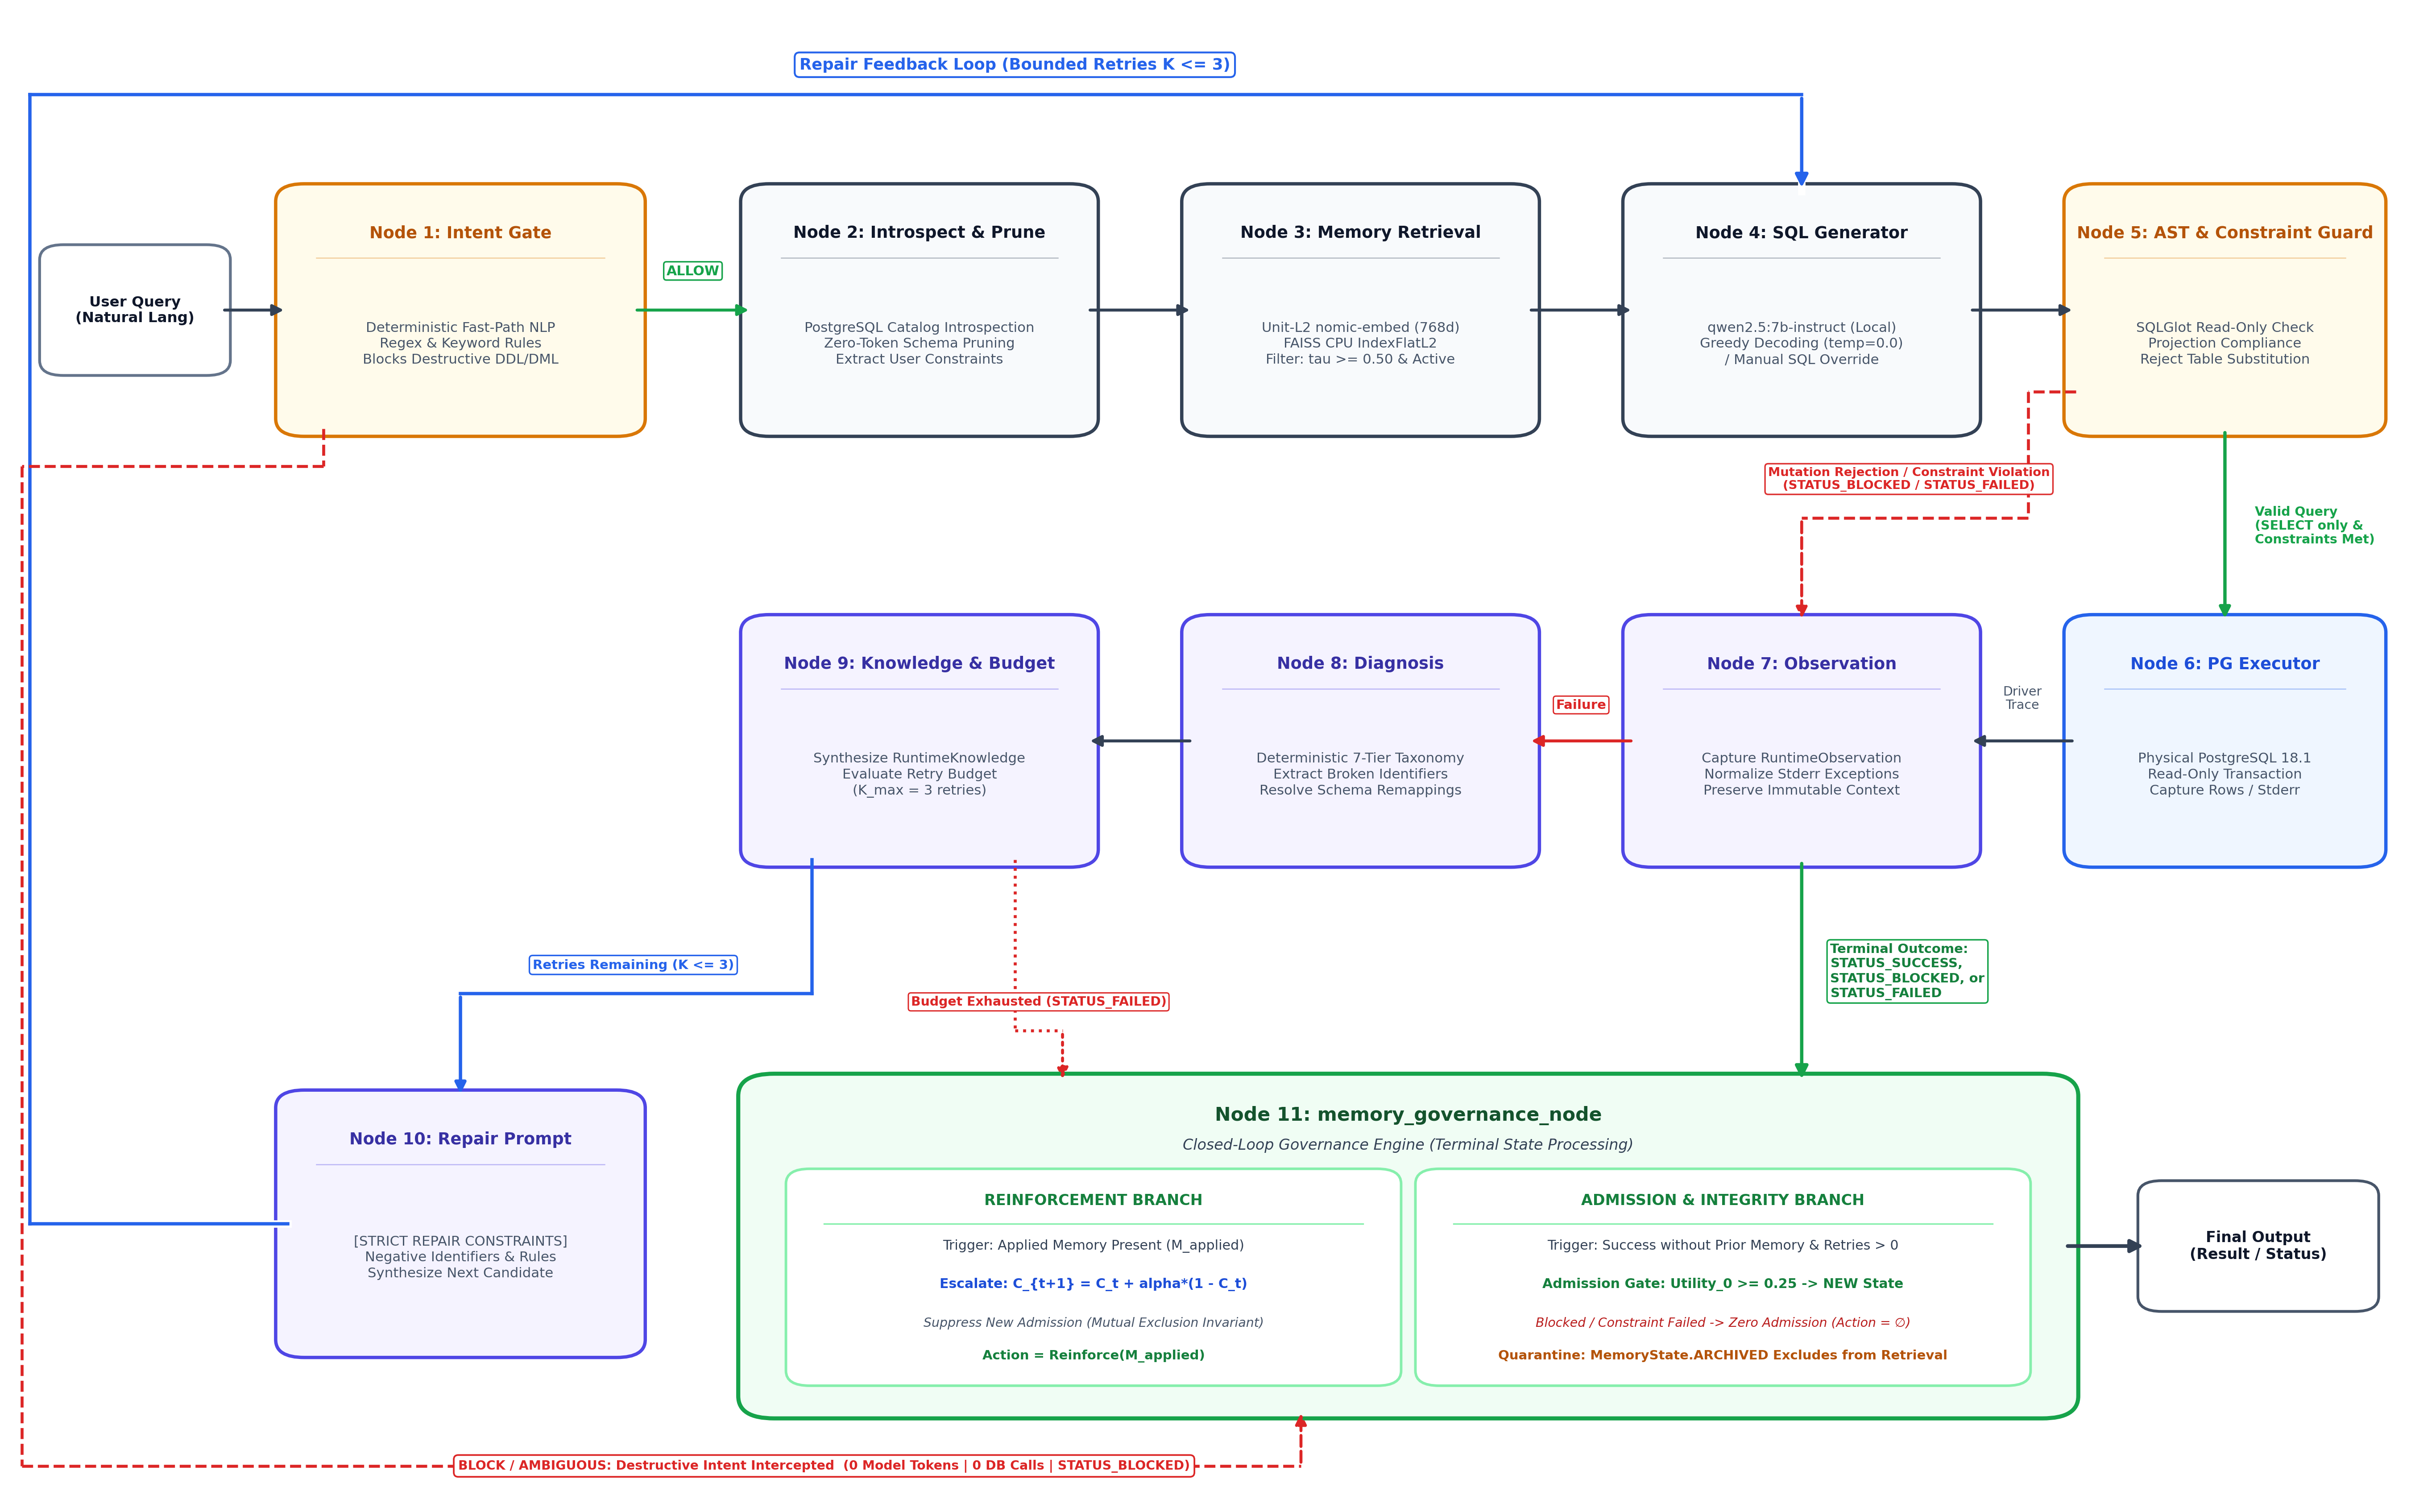
\includegraphics[width=\textwidth]{fig1_architecture.png}
\caption{ARMG 11-Node LangGraph Architecture and Closed-Loop State Machine. The diagram shows the complete post-v1.0 workflow: entry intent gating (Node 1) and explicit user-constraint checks (Nodes 2 and 5) were added after the frozen v1.0 benchmark and evaluated in separate test suites, whereas the v1.0 benchmark exercised schema pruning, FAISS retrieval, SQL generation, SQLGlot AST safety validation, read-only PostgreSQL execution, bounded 7-tier repair ($K \le 3$), and mutual-exclusion memory governance.}
\label{fig:architecture}
\end{figure*}

\subsection{Prompt Guidance vs. Deterministic Enforcement}
Table~\ref{tab:enforcement} separates prompt-level guidance, heuristic rules, parser validation, database-session settings, and governance state transitions. Negative constraints $\mathcal{N}_k$ are inserted into the repair prompt inside \texttt{[STRICT REPAIR CONSTRAINTS]} without a post-generation identifier blacklist: they influence token generation without guaranteeing that the model obeys them, and we do not treat that prompt block as a deterministic safety gate (Section~\ref{sec:ablation}).

\begin{table*}[t]
\centering
\caption{Enforcement Mechanism and Actual Guarantee Scope for Each System Restriction}
\label{tab:enforcement}
\footnotesize
\setlength{\tabcolsep}{4pt}
\renewcommand{\arraystretch}{1.05}
\begin{tabularx}{\textwidth}{@{}>{\raggedright\arraybackslash}p{3.1cm} >{\raggedright\arraybackslash}p{3.9cm} >{\raggedright\arraybackslash}p{2.8cm} >{\raggedright\arraybackslash}X@{}}
\toprule
\textbf{Restriction} & \textbf{Implemented Mechanism} & \textbf{Enforcement Type} & \textbf{Guarantee and Scope Boundary} \\
\midrule
Destructive or ambiguous natural-language prompt & Keyword and regex intent classifier (\url{validation/intent_classifier.py}) & Deterministic check on heuristic lexical rules & Halts phrasings matched by the implemented rule set (post-v1.0); provides no guarantee against obfuscated or paraphrased prompts \\
Non-\texttt{SELECT} root or stacked multi-statement SQL & SQLGlot statement-count and root-type check (\url{validation/execution_validator.py}) & Deterministic static parse check & Rejects multi-statement inputs and non-\texttt{SELECT} statement roots parsed by SQLGlot (PostgreSQL dialect); does not block valid-\texttt{SELECT} resource amplification \\
User-mandated tables, prohibited tables, and output columns & Constraint extractor and \texttt{SELECT}-projection checker (\url{validation/constraint_validator.py}) & Deterministic check on heuristically extracted constraints & Rejects missing \texttt{SELECT} projections, disallowed \texttt{SELECT *} wildcards, and prohibited tables (post-v1.0), bounded by heuristic text-extraction coverage \\
Broken identifiers in $\mathcal{N}_k$ during repair & \texttt{[STRICT REPAIR CONSTRAINTS]} prompt section & Prompt-level text guidance & Influences LLM regeneration only; no post-generation blacklist guarantees model compliance \\
Database writes and long single-query execution & PostgreSQL read-only session settings and statement timeout (\url{environment/postgres.py}) & Database-session enforcement & Enforces a read-only database boundary in that session and cancels single queries exceeding the timeout; concurrent load exhaustion was not tested \\
Admission, reinforcement, or penalty of repair records & Governance state rules and archive API (\url{memory/governance.py}) & Deterministic state rule & Deterministically decides whether a record is admitted, reinforced, penalized, or unchanged; \texttt{ARCHIVED}/\texttt{DELETED} records are excluded from retrieval \\
\bottomrule
\end{tabularx}
\end{table*}

\section{Safety Evaluation}
\label{sec:safety}
\subsection{Threat Boundaries and Workflow Routing}
ARMG enforces five separate boundaries: the post-v1.0 rule-based intent gate (Layer~1); the SQLGlot AST guard requiring statement count $= 1$ and a \texttt{SELECT} root expression (Layer~2); the post-v1.0 user-constraint validator checking mandated \texttt{SELECT} column projections, rejecting \texttt{SELECT *} when specific output columns are requested, and blocking prohibited table substitutions (Layer~3); read-only PostgreSQL session parameters with bounded statement timeouts (Layer~4); and governed memory admission paired with the administrative \texttt{quarantine\_\allowbreak{}memory\_\allowbreak{}by\_\allowbreak{}id} archival API (Layer~5).

Failures route along distinct paths: matched destructive or ambiguous prompts (Layer~1) and non-\texttt{SELECT} or multi-statement AST candidates (Layer~2) halt immediately in \texttt{STATUS\_\allowbreak{}BLOCKED} without calling PostgreSQL; user-constraint rejections (Layer~3) enter bounded repair without calling PostgreSQL; and unknown identifiers inside syntactically valid \texttt{SELECT} queries reach PostgreSQL (Layer~4) and route driver errors to diagnosis. Controlled manual SQL overrides in test harnesses bypass Layer~1 to test downstream boundaries directly.

\subsection{Separated Verification Scopes}
Because Layers~1 and~3 were added after the frozen v1.0 benchmark, Table~\ref{tab:safety_scopes} reports every verification scope separately rather than combining them into a universal security claim. The five live PostgreSQL integration tests (\texttt{test\_\allowbreak{}repair\_\allowbreak{}integration.py}) test manual override routing, AST validation, PostgreSQL error capture, Tier~3 semantic repair, and memory admission (Layers~2, 4, and~5), whereas Layer~3 constraint checks are covered by their dedicated 23-test unit suite.

\begin{table*}[t]
\centering
\caption{Safety, Compliance, and Lifecycle Verification Evidence Separated by Evaluation Scope}
\label{tab:safety_scopes}
\footnotesize
\setlength{\tabcolsep}{4pt}
\renewcommand{\arraystretch}{1.05}
\begin{tabularx}{\textwidth}{@{}>{\raggedright\arraybackslash}p{3.5cm} c >{\raggedright\arraybackslash}p{2.8cm} >{\raggedright\arraybackslash}X@{}}
\toprule
\textbf{Evaluation Scope} & \textbf{Target Component} & \textbf{Reported Scope} & \textbf{Appropriate Conclusion and Boundary} \\
\midrule
Frozen primary benchmark (v1.0) & Layers 2, 4, 5 & 450 query-level evaluations (18 runs) & Zero unintended warehouse mutations recorded in this benign analytical workload; predates Layers 1 and 3 and does not test adversarial prompts \\
Phase 10 static SQL AST audit & Layer 2 (SQLGlot) & 33 SQL cases (12 controls, 21 unsafe) & All 21 tested unsafe variants blocked (\texttt{DROP}, \texttt{DELETE}, \texttt{UPDATE}, \texttt{INSERT}, \texttt{ALTER}, \texttt{TRUNCATE}, \texttt{GRANT}, \texttt{REVOKE}, transaction blocks, stacked statements, comment-hidden mutations) and all 12 controls accepted \\
Intent-gate unit tests (post-v1.0) & Layer 1 (Intent) & 37 unit tests & All 37 tested rule-based destructive and ambiguous intent cases passed (\texttt{STATUS\_BLOCKED}, zero LLM tokens, zero DB calls) \\
User-constraint unit tests (post-v1.0) & Layer 3 (Constraints) & 23 unit tests & All 23 tested explicit table-prohibition, missing-\texttt{SELECT}-column, and disallowed-\texttt{SELECT *} cases passed \\
AST safety unit tests & Layer 2 (SQLGlot) & 59 unit tests (two modules) & All 59 tested single-statement and non-\texttt{SELECT} AST rejection cases passed \\
Live PostgreSQL integration tests & Layers 2, 4, 5 & 5 live DB integration tests & All 5 tested integration workflows passed, including single-call manual-override failure ($K=0$) and live \texttt{revenue} $\to$ \texttt{gross\_revenue} repair ($K=1$) with admission \\
Temporal-decay simulation harness & Lifecycle decay eq. & 63 simulated-time conditions & The stated decay equation and archival transitions passed all simulated-time checks (0--60 days); does not test live multi-day retrieval quality \\
\bottomrule
\end{tabularx}
\end{table*}

\section{Runtime Observation and Error Diagnosis}
\subsection{The 7-Tier Taxonomy and Pre-Execution Rejections}
In our implementation, \texttt{DiagnosticEngine} deterministically maps each normalized observation into one of seven tiers (Table~\ref{tab:taxonomy}). Rejections produced at Node~5 \emph{before} PostgreSQL submission---both AST safety blocks and user-constraint failures---are assigned to Tier~1 (\texttt{Validation}). Tier~5 (\texttt{Permission}) is assigned only when a query passes Node~5 and PostgreSQL itself raises a permission or read-only transaction exception at Node~6; accordingly, an administrative \texttt{GRANT} statement stopped by SQLGlot is recorded as a Tier~1 validation rejection rather than a Tier~5 server error.

\begin{table*}[t]
\centering
\caption{Canonical 7-Tier Exception Taxonomy and Candidate Repair Actions}
\label{tab:taxonomy}
\footnotesize
\setlength{\tabcolsep}{4pt}
\renewcommand{\arraystretch}{1.04}
\begin{tabularx}{\textwidth}{@{}c l >{\raggedright\arraybackslash}p{3.5cm} >{\raggedright\arraybackslash}p{4.1cm} >{\raggedright\arraybackslash}X@{}}
\toprule
\textbf{Tier} & \textbf{Category} & \textbf{Implementation Definition} & \textbf{Detection Pattern / Trigger} & \textbf{Workflow Routing / Candidate Repair Action} \\
\midrule
1 & Validation & Pre-execution AST or user-constraint rejections & Non-\texttt{SELECT} AST root, multi-statement SQL, or explicit constraint violation at Node 5 & AST violations abort to \texttt{STATUS\_BLOCKED}; constraint violations enter bounded repair \\
2 & Syntax & Malformed SQL grammar & PostgreSQL syntax errors, unclosed quotes, malformed clauses & Strip invalid tokens; regenerate with PostgreSQL grammar \\
3 & Semantic & Catalog identifier non-existence or ambiguity & Unknown column or table names, ambiguous column references & Score catalog replacement tokens; place broken token in $\mathcal{N}_k$ \\
4 & Planning & Missing or invalid join predicates & Unbounded joins or invalid foreign-key comparisons & Suggest direct single-hop \texttt{JOIN ... ON} key from catalog \\
5 & Permission & Server-raised privilege or read-only errors & PostgreSQL permission or read-only transaction rejections at Node 6 & Halt write attempt; restrict candidate to read-only \texttt{SELECT} \\
6 & Resource & Execution timeout or memory cancellation & Statement timeout cancellation or server memory limit exceeded & Enforce statement timeout; suggest predicate pushdown \\
7 & Execution & Unclassified runtime driver exceptions & Remaining runtime driver errors (e.g., division by zero, cast failure) & Pass normalized driver error trace to repair prompt \\
\bottomrule
\end{tabularx}
\end{table*}

\subsection{Heuristic Candidate Scoring: Rationale, Formula Illustration, and Limits}
When PostgreSQL raises a Tier~3 \texttt{Semantic} error on an unknown column $c_{\text{broken}}$, \texttt{DiagnosticEngine} scores candidate columns $c_{\text{cand}}$ from $\mathcal{S}_q$ without an LLM call by summing five features designed by our team during initial schema prototyping: $+10.0$ if $c_{\text{broken}}$ is a substring of $c_{\text{cand}}$; $+8.0$ per shared underscore-delimited token; $+4.0 \times \text{difflib.SequenceMatcher.ratio()}$; $+6.0$ when $c_{\text{cand}}$ has a numeric data type matching a metric query; and manually specified sales-domain priors of $+15.0$ for \texttt{revenue} $\to$ \texttt{gross\_\allowbreak{}revenue} and $+10.0$ for \texttt{revenue} $\to$ \texttt{net\_\allowbreak{}profit}. Exact ties are broken alphabetically by identifier, and top-ranked candidates populate \texttt{candidate\_\allowbreak{}replacements} in the repair prompt rather than rewriting the SQL AST directly.

These numerical weights were assigned during schema prototyping prior to benchmark execution. To illustrate candidate ranking, consider a representative calculation for $c_{\text{broken}} = \texttt{revenue}$ (length 7) on \texttt{fact\_sales\_performance} under numeric metric affinity:
\begin{itemize}
\item \texttt{gross\_revenue} (length 13; contiguous match length 7, ratio $2 \times 7 / (7 + 13) = 0.70$): $10.0\text{ (substring)} + 8.0\text{ (token \texttt{revenue})} + 4.0 \times 0.70 + 6.0\text{ (numeric)} + 15.0\text{ (sales prior)} = 41.80$.
\item \texttt{net\_profit} (length 10; single-character match \texttt{'r'}, ratio $2 \times 1 / (7 + 10) = 2/17 \approx 0.1176$): $0 + 0 + 4.0 \times (2/17) + 6.0 + 10.0 \approx 16.47$.
\item \texttt{units\_sold} (length 10; single-character match \texttt{'n'}, ratio $2/17 \approx 0.1176$): $0 + 0 + 4.0 \times (2/17) + 6.0 + 0 \approx 6.47$.
\end{itemize}
Although \texttt{gross\_revenue} ranks highest under these weights, the scoring logic depends on surface lexical overlap and domain-specific affinity rules, constraining its transferability across schemas with dissimilar naming conventions or non-commercial schemas.

\subsection{Ephemeral Runtime-Knowledge}
Diagnostic findings $\Delta_k$ are packaged into an immutable \texttt{Runtime-Knowledge} record storing \texttt{failure\_\allowbreak{}type}, \texttt{source\_\allowbreak{}exception}, \texttt{context}, \texttt{root\_\allowbreak{}cause}, \texttt{repair\_\allowbreak{}strategy}, \texttt{negative\_\allowbreak{}constraints}, \texttt{candidate\_\allowbreak{}replacements}, initial confidence $C_0 = 0.50$, and UTC timestamp. During repair, Node~10 supplies $\mathcal{S}_q$, $q$, failed SQL $s_{k-1}$, normalized error $\bar{e}_{k-1}$, the \texttt{[STRICT REPAIR CONSTRAINTS]} prompt block, and retrieved memory rules $\mathcal{M}_{\text{ret}}$.

\section{Memory Governance and Lifecycle}
\label{sec:governance}
\subsection{Operational Utility, Recency, and Confidence Decay}
\label{sec:decay_authoritative}
Our governance equations in \url{memory/governance.py} compute operational utility as
\begin{equation}
\begin{aligned}
\text{Utility} = {} & C \times \text{SuccessRate} \\
& \times \text{ContextSimilarity} \times \text{Recency}
\end{aligned}
\end{equation}
where $\text{SuccessRate} = \text{successful\_uses}/\text{total\_uses}$ (initialized to prior $0.50$ before reuse), $\text{ContextSimilarity} = 1/(1+d^2)$ from squared FAISS $L_2$ distance $d^2$ \cite{johnson2021faiss}, and
\begin{equation}
\text{Recency} = \frac{1}{1 + \Delta t}, \qquad C(t) = C_{\text{ref}} \exp(-\lambda \Delta t)
\end{equation}
for elapsed time $\Delta t \ge 0$ in days. In our implementation, elapsed time $\Delta t$ enters $\text{Utility}$ twice: once via the query-time $\text{Recency}$ weight and once via exponential decay of stored confidence $C(t)$, which drives lifecycle transitions into \texttt{DECAYING} and \texttt{ARCHIVED} ($C < 0.20$). Including both time-dependent terms is an unvalidated design choice whose combined effect was not systematically evaluated. Because each 25-query benchmark run completed in approximately 3.5 minutes ($\Delta t \approx 0.002$ days), both factors remained near unity ($\exp(-0.05 \times 0.002) \approx 0.9999$ and $\text{Recency} \approx 0.9980$). The live benchmark therefore cannot establish whether multi-day decay improves retrieval quality; our 63-condition simulated-time harness ($9\text{ initial confidence levels} \times 7\text{ intervals from 0 to 60 days}$) validates the mathematical formulation and state transitions, not live multi-day retrieval performance.

Because stored embeddings are unit-$L_2$ normalized ($d^2 = 2 - 2\cos\theta$), the retrieval cutoff $S = 1/(1+d^2) \ge \tau = 0.50$ is equivalent to $d^2 \le 1.0$ ($\cos\theta \ge 0.50$). Observed Mode 4 similarity scores ($0.4755$ to $0.5388$; Table~\ref{tab:fig3_validation}) cluster near $0.50$, making retrieval membership sensitive to the exact setting of $\tau$.

\subsection{Governance Parameter Status}
Table~\ref{tab:params} summarizes all governance parameters. No systematic sensitivity analysis was conducted to optimize these thresholds: all defaults were fixed manually before freezing the v1.0 benchmark, and only $\lambda$ was changed in Mode 6 ($0.05\text{ day}^{-1}$ vs. $0.0$).

\begin{table}[t]
\centering
\caption{Governance Parameter Values and Experimental Status}
\label{tab:params}
\footnotesize
\setlength{\tabcolsep}{3pt}
\renewcommand{\arraystretch}{1.04}
\begin{tabularx}{\columnwidth}{@{}>{\raggedright\arraybackslash}p{2.7cm} c >{\raggedright\arraybackslash}X@{}}
\toprule
\textbf{Parameter} & \textbf{Value} & \textbf{Experimental Status in This Study} \\
\midrule
Initial priors ($C_0, \text{SR}_0$) & 0.50, 0.50 & Fixed pre-benchmark; not varied \\
Admission threshold $\theta_{\text{admit}}$ & 0.25 & Fixed pre-benchmark; equals $\text{Utility}_0 = 0.25$ for every new record (non-selective numerically) \\
Retrieval threshold $\tau$ & 0.50 & Fixed pre-benchmark; observed scores lie near $0.50$, sensitivity untested \\
Confidence gain $\alpha$ & 0.10 & Fixed pre-benchmark; not varied \\
Failure penalty $\beta$ & 0.15 & Fixed pre-benchmark; not varied \\
Lifecycle cutoffs (\texttt{ARCHIVED}, \texttt{STABLE}) & 0.20, 0.80 & Fixed pre-benchmark; state transitions verified in unit and simulation tests \\
Decay rate $\lambda$ & 0.05/day & Varied only in Mode 6 ($0.0$ vs. $0.05$; see Section~\ref{sec:decay_authoritative}) \\
\bottomrule
\end{tabularx}
\end{table}

\subsection{Structural Admission Preconditions and Non-Selectivity of the Utility Threshold}
Every new \texttt{Runtime-Knowledge} record is initialized with $C_0 = 0.50$, $\text{SR}_0 = 0.50$, $\text{ContextSimilarity} = 1.0$, and $\text{Recency} = 1.0$, yielding $\text{Utility}_0 = 0.25$, which is exactly equal to $\theta_{\text{admit}} = 0.25$. Under this initialization, the numerical comparison $\text{Utility}_0 \ge \theta_{\text{admit}}$ is satisfied with equality by every newly synthesized repair artifact and does not distinguish or filter candidate rules. Actual admission selectivity in ARMG comes entirely from the structural preconditions in Eq.~\eqref{eq:governance_action}: an initial SQL attempt must fail, a subsequent repair attempt must succeed after at least one retry ($K \ge 1$), and no persistent memory may have been applied during that repair episode ($M_{\text{applied}} = \emptyset$).

To align the formal governance rule with the logged benchmark events (Table~\ref{tab:fig6_validation}), we distinguish \emph{retrieved memory} ($\mathcal{M}_{\text{ret}}$, entries returned at Node~3 for the initial prompt) from \emph{memory applied in repair} ($M_{\text{applied}}$, retrieved entries active during a repair cycle with $K \ge 1$). When a query retrieves entries at Node~3 ($\mathcal{M}_{\text{ret}} \neq \emptyset$) and succeeds on Attempt~1 without entering repair ($K = 0$, as on Q10, Q16, Q18, Q20--Q25, and seed-42 Q19), no repair episode occurs ($M_{\text{applied}} = \emptyset$ and $K = 0$), so Node~11 leaves the store unchanged. When a query fails initially and enters repair ($K \ge 1$) with retrieved entries present ($M_{\text{applied}} = \mathcal{M}_{\text{ret}} \neq \emptyset$, as on Q08, Q17, and seeds-123/999 Q19), those entries constitute applied memories for that repair episode. Repairs where $K \ge 1$ and $\mathcal{M}_{\text{ret}} = \emptyset$ (Q04, Q13, and Q15) succeed using PostgreSQL error messages and diagnostic prompts without persistent memory injection, satisfying the admission condition.

\begin{table*}[t]
\centering
\caption{Governance Control Equations and Lifecycle State Transitions}
\label{tab:governance_equations}
\footnotesize
\setlength{\tabcolsep}{4pt}
\renewcommand{\arraystretch}{1.05}
\begin{tabularx}{\textwidth}{@{}>{\raggedright\arraybackslash}p{2.7cm} >{\raggedright\arraybackslash}p{5.3cm} >{\raggedright\arraybackslash}p{3.7cm} >{\raggedright\arraybackslash}X@{}}
\toprule
\textbf{Control Mechanism} & \textbf{Formal Expression} & \textbf{Trigger Precondition} & \textbf{Store / Lifecycle State Effect} \\
\midrule
Operational Utility & $\text{Utility} = C \times \text{SuccessRate} \times \text{ContextSim} \times \text{Recency}$ & Candidate scoring (note: $\Delta t$ enters via both $C$ and $\text{Recency}$) & Ranks stored memories using confidence, empirical reuse rate, $L_2$ similarity, and recency \\
Repair-Rule Admission & $\text{Admit}(K_{\text{new}})$ (with $\text{Utility}_0 = \theta_{\text{admit}} = 0.25$) & Initial fail $\land$ $\text{STATUS\_SUCCESS} \land K \ge 1 \land M_{\text{applied}} = \emptyset$ & Admits new vector record in state \texttt{NEW}; selectivity stems from structural preconditions \\
Confidence Escalation & $C_{t+1} = C_t + \alpha (1.0 - C_t)$ & $\text{STATUS\_SUCCESS} \land K \ge 1 \land M_{\text{applied}} \neq \emptyset$ & Reinforces applied memory (\texttt{NEW} $\to$ \texttt{ACTIVE}; \texttt{STABLE} at $C \ge 0.80$); suppresses admission \\
Failure Penalty & $C_{t+1} = \max(0.0, \, C_t (1.0 - \beta))$ & $\text{STATUS\_FAILED} \land M_{\text{applied}} \neq \emptyset$ & Penalizes applied memory (\texttt{ARCHIVED} if $C_{t+1} < 0.20$); suppresses admission \\
Continuous Decay\textsuperscript{a} & $C(t) = C_{\text{ref}} \exp(-\lambda \Delta t)$ & Elapsed time $\Delta t > 0$ (days) & Decays $C(t)$ toward \texttt{ARCHIVED} ($C < 0.20$) and 30-day \texttt{DELETED} purge \\
\bottomrule
\end{tabularx}
\vspace{2.0pt}
\begin{minipage}{\textwidth}
\footnotesize \textsuperscript{a}See Section~\ref{sec:decay_authoritative} for simulated-time verification and live benchmark duration bounds.
\end{minipage}
\end{table*}

\subsection{Mutual Exclusion Between Applied-Memory Updates and New Admission}
At terminal outcomes across retry count $K \in \{0, 1, 2, 3\}$, Node~11 executes one of four mutually exclusive branches (Table~\ref{tab:governance_equations}; Fig.~\ref{fig:lifecycle}):
\begin{equation}
\label{eq:governance_action}
\text{Action} = \begin{cases}
\text{Reinforce}(M_{\text{applied}}), & \text{if } \text{Success} \land K \ge 1 \\
& \quad \land \; M_{\text{applied}} \neq \emptyset, \\
\text{Admit}(K_{\text{new}}), & \text{if } \text{Success} \land K \ge 1 \\
& \quad \land \; M_{\text{applied}} = \emptyset, \\
\text{Penalize}(M_{\text{applied}}), & \text{if } \text{Failed} \land M_{\text{applied}} \neq \emptyset, \\
\emptyset, & \text{otherwise.}
\end{cases}
\end{equation}
The fourth branch ($\emptyset$) leaves the store unchanged on first-attempt successes ($K = 0$), pre-execution blocks (\texttt{STATUS\_BLOCKED}), and terminal repair failures where no memory was applied ($M_{\text{applied}} = \emptyset$, rejected as \texttt{TERMINAL\_FAILURE\_NOT\_ADMITTED}). Whenever an existing memory is applied during repair ($M_{\text{applied}} \neq \emptyset$), Node~11 reinforces its confidence on repair success or penalizes its confidence on terminal repair failure while suppressing new admission in that episode. This mutual-exclusion invariant bounds store growth on recurring errors, with the trade-off that a partially matching applied memory suppresses admission of a new rule during that episode.

\begin{figure}[t]
\centering
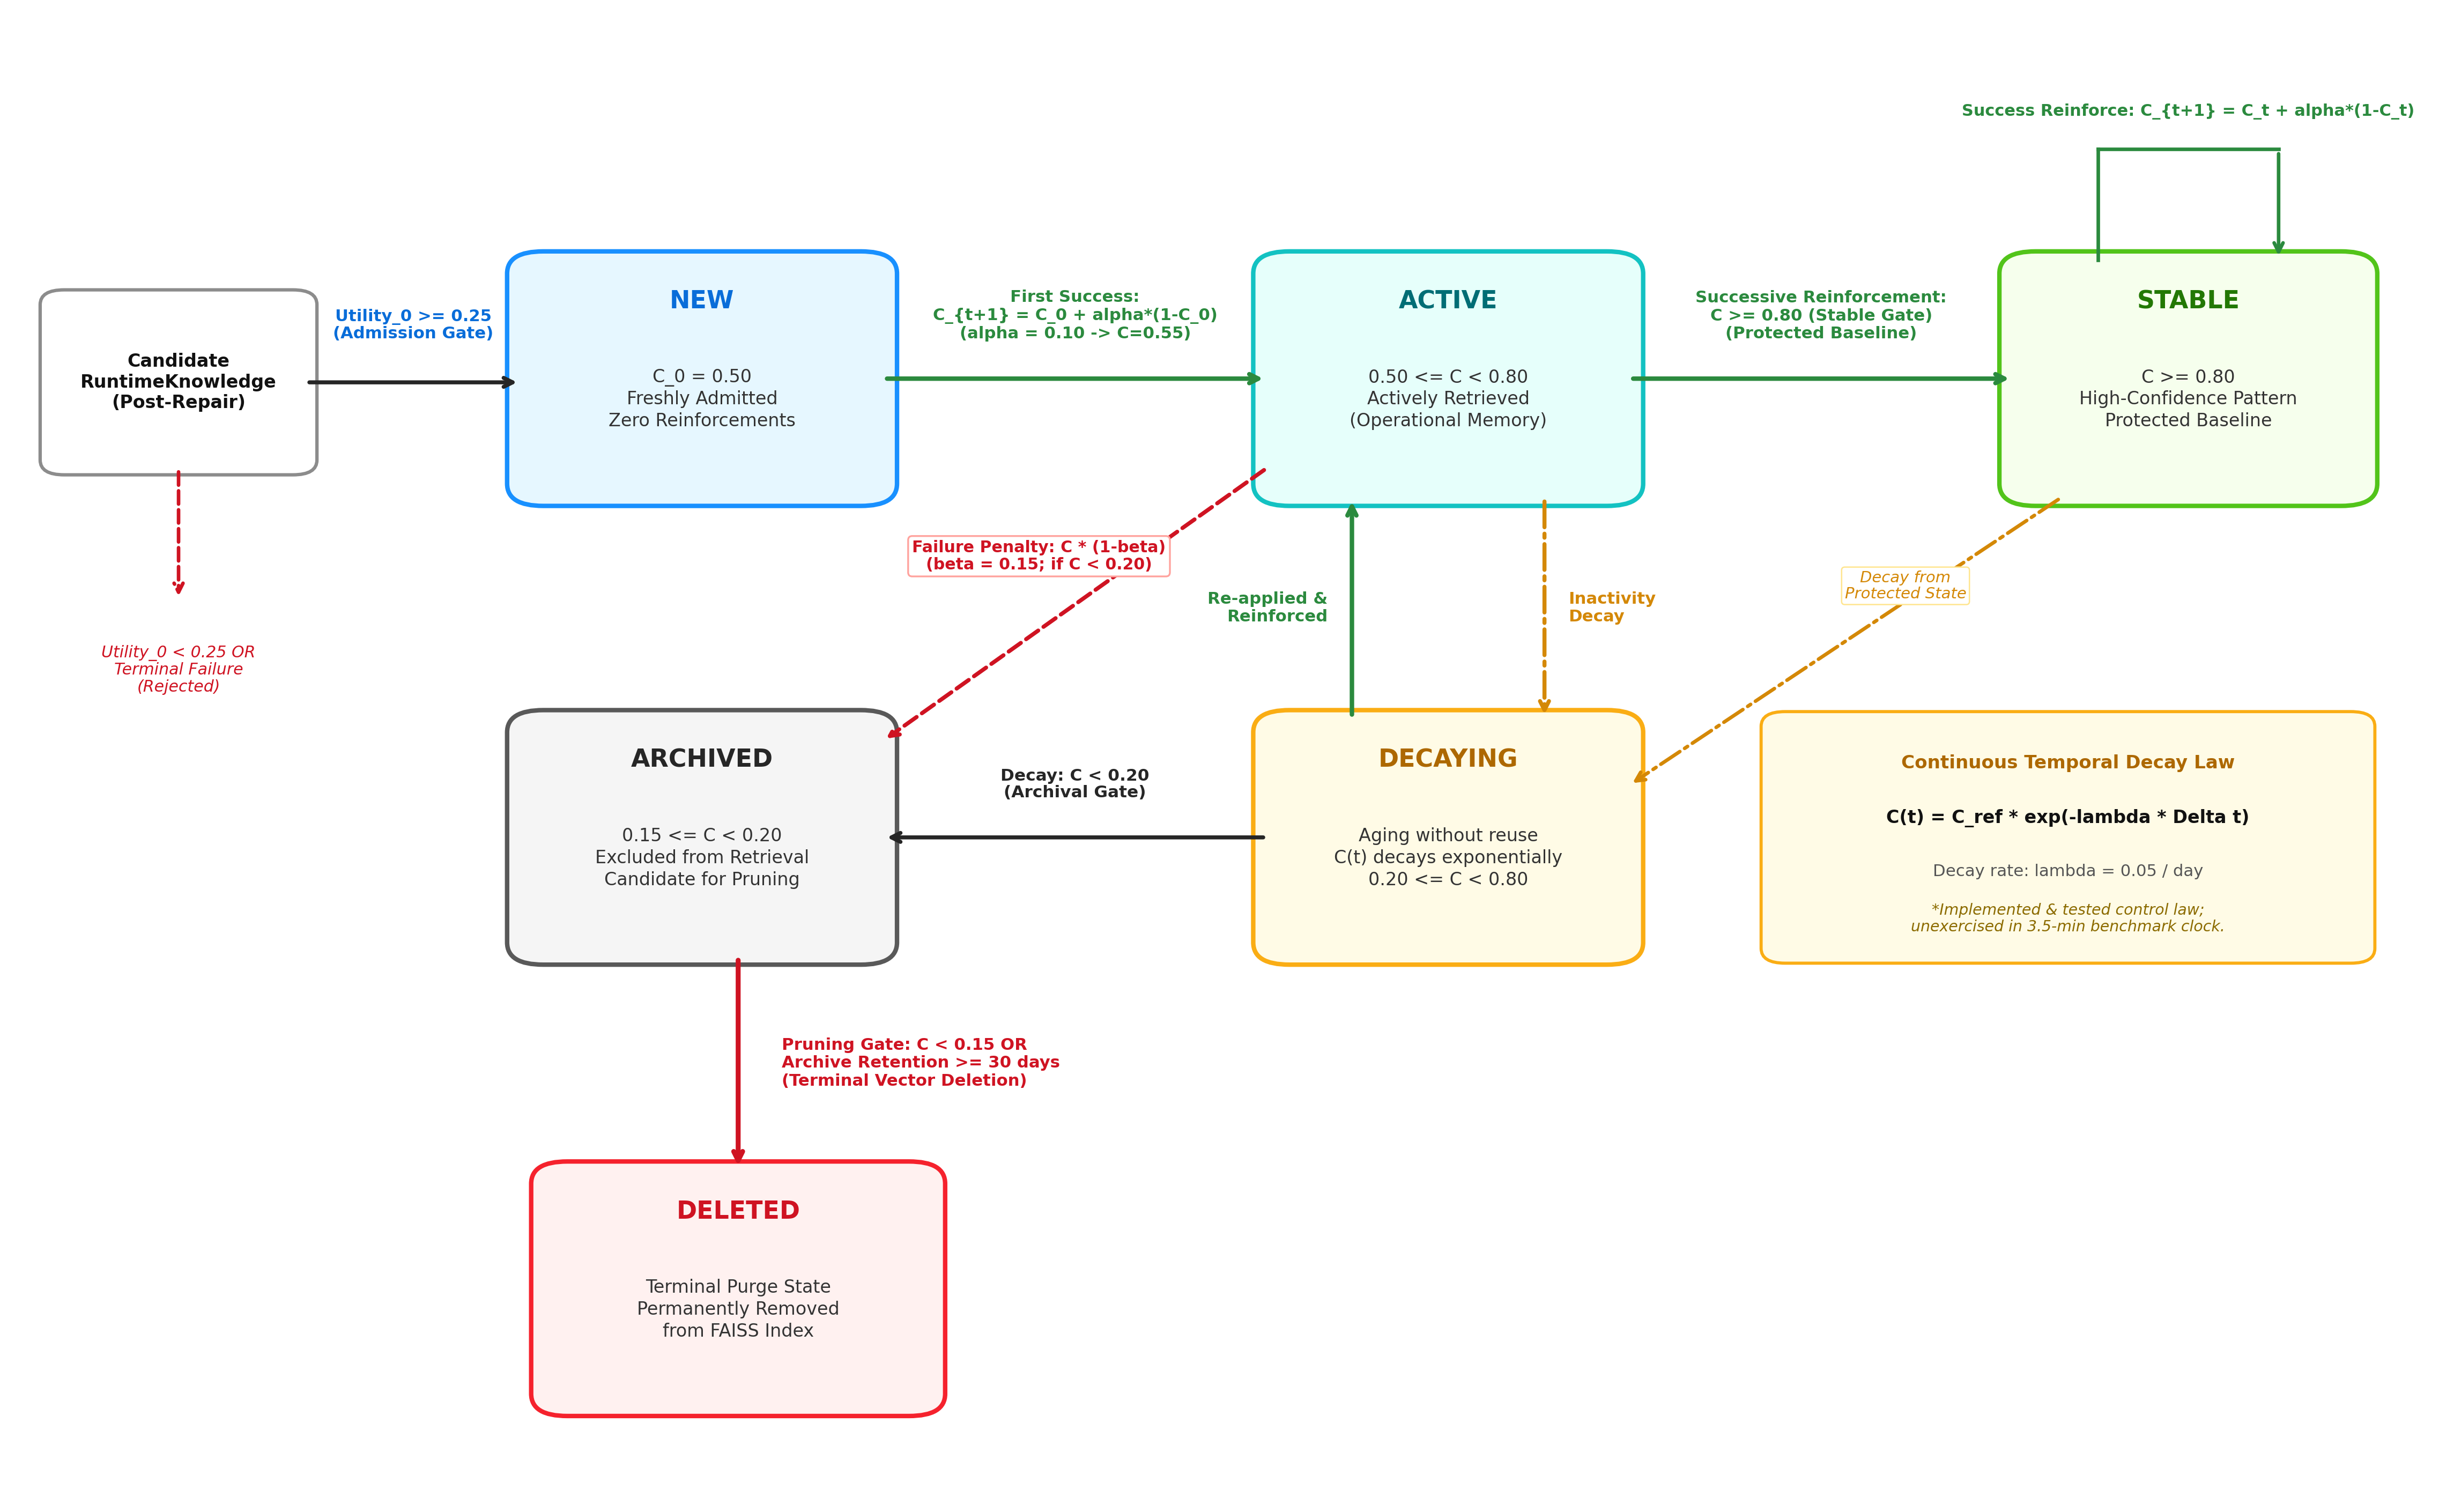
\includegraphics[width=\columnwidth]{fig2_lifecycle.png}
\caption{Runtime Memory Lifecycle State Transition Machine across six discrete states (\texttt{NEW}, \texttt{ACTIVE}, \texttt{STABLE}, \texttt{DECAYING}, \texttt{ARCHIVED}, \texttt{DELETED}), governed by structural repair-admission preconditions ($K \ge 1, M_{\text{applied}}=\emptyset$, with $\text{Utility}_0 = \theta_{\text{admit}} = 0.25$), asymptotic reinforcement ($\alpha = 0.10$), failure penalty ($\beta = 0.15$), archival cutoff ($C < 0.20$), exponential decay ($\lambda = 0.05/\text{day}$), and 30-day archive deletion.}
\label{fig:lifecycle}
\end{figure}

\section{Experimental Methodology}
\subsection{Terminology and Evaluation Scopes}
A \emph{run} is one complete sequential pass over the 25 benchmark queries under a single mode and seed. Six modes evaluated across three seeds (42, 123, and 999) produce 18 runs and $18 \times 25 = 450$ \emph{query-level evaluations}, all recorded on the frozen ARMG v1.0 pipeline. While \texttt{pytest --collect-only} discovers 489 test definitions across the repository (456 unit, 21 integration, and 12 environment tests), we do not claim all 489 discovered tests as executed safety evidence; the safety, constraint, and lifecycle results reported in this paper rest strictly on the separated scopes itemized in Table~\ref{tab:safety_scopes} (the 450-evaluation frozen benchmark, the 33-case static AST audit, the 37 intent-gate, 23 constraint, and 59 AST unit tests, the 5 live PostgreSQL integration tests, and the 63-condition simulated-time decay harness).

\subsection{Experimental Design Rationale}
\textbf{Shared synthetic Star Schema.} Tracking whether repair rules extracted from early execution errors are admitted, retrieved, and reinforced on subsequent queries requires a shared warehouse schema across a known sequence. We built a synthetic four-table B2B sales Star Schema (Table~\ref{tab:schema}; deterministically seeded with 2,000 fact rows via NumPy \texttt{seed=42} in \url{scripts/seed_warehouse.py}) on PostgreSQL 18.1 (Table~\ref{tab:system_config}) containing recurring column-naming traps (e.g., ``revenue'' vs. \texttt{gross\_revenue} and \texttt{net\_profit}) and multi-table dimension joins. This controlled single-schema design enables exact store-trajectory verification while limiting external validity across broader schemas.

\textbf{Sequential query categories.} The 25 analytical queries (\url{benchmark/queries.json}; Table~\ref{tab:query_corpus}) execute in fixed sequential order Q01--Q25 across four categories: single-table aggregations and ordering in Category~A (Q01--Q05), Star Schema joins in Category~B (Q06--Q13), window functions in Category~C (Q14--Q19), and column-naming traps and strict projection orderings in Category~D (Q20--Q25).

\textbf{Repeated greedy executions and descriptive statistics.} All modes ran under greedy decoding (\texttt{temperature = 0.0}, \texttt{top\_p = 1.0}). Because greedy decoding is not a stochastic sampling distribution, the three runs per mode inspect pipeline repeatability rather than sampling variance, and reported means and sample standard deviations ($n = 3$ runs) are purely descriptive summaries rather than inferential significance tests.

\begin{table}[t]
\centering
\caption{System Configuration and Component Mapping}
\label{tab:system_config}
\footnotesize
\setlength{\tabcolsep}{2.5pt}
\renewcommand{\arraystretch}{1.03}
\begin{tabularx}{\columnwidth}{@{}p{2.1cm} p{2.0cm} >{\raggedright\arraybackslash}X@{}}
\toprule
\textbf{Subsystem} & \textbf{Anchor} & \textbf{Specification} \\
\midrule
Foundation Model & Local Ollama & \texttt{qwen2.5:\allowbreak{}7b-\allowbreak{}instruct} (7.61B) \\
Inference Config & Local Ollama & Greedy (\texttt{temp=\allowbreak{}0.0}, \texttt{top\_p=\allowbreak{}1.0}) \\
Embedding Model & Local Ollama & \texttt{nomic-\allowbreak{}embed-\allowbreak{}text} (768d, Unit-$L_2$) \\
Vector Index & CPU Flat Index & FAISS \texttt{Index\allowbreak{}IDMap2} (\texttt{Index\allowbreak{}FlatL2}) \\
Warehouse & Container & PostgreSQL 18.1 on \texttt{localhost:\allowbreak{}5432} \\
Graph Engine & Directed Graph & LangGraph 0.2.x (\texttt{State\allowbreak{}Graph}) \\
Static Parser & AST Guardrail & SQLGlot 25.x (Dialect: PostgreSQL) \\
Driver & DB-API 2.0 & \texttt{psycopg2-\allowbreak{}binary} 2.9.x \\
Runtime & Workstation & Python 3.13.2 (system) / 3.11.9 (.venv) \\
\bottomrule
\end{tabularx}
\end{table}

\begin{table*}[t]
\centering
\caption{Synthetic PostgreSQL Star Schema Specification}
\label{tab:schema}
\footnotesize
\setlength{\tabcolsep}{5pt}
\renewcommand{\arraystretch}{1.03}
\begin{tabularx}{\textwidth}{@{}l c c l >{\raggedright\arraybackslash}X@{}}
\toprule
\textbf{Table Name} & \textbf{Role} & \textbf{Rows} & \textbf{Primary Key} & \textbf{Major Attributes and Foreign Key Constraints} \\
\midrule
\texttt{dim\_time} & Dimension & 365 & \texttt{time\_key} & full\_date, day\_of\_week, calendar\_month, calendar\_quarter, calendar\_year \\
\texttt{dim\_geography} & Dimension & 6 & \texttt{geo\_key} & region, zone, market\_type \\
\texttt{dim\_product} & Dimension & 8 & \texttt{product\_key} & product\_name, category, sub\_category, unit\_cost \\
\texttt{fact\_sales\_performance} & Fact & 2,000 & \texttt{fact\_key} & units\_sold, gross\_revenue, discount\_applied, net\_profit. \newline FK: \texttt{time\_key}, \texttt{geo\_key}, \texttt{product\_key} \\
\bottomrule
\end{tabularx}
\vspace{2.0pt}
\begin{minipage}{\textwidth}
\footnotesize \textsuperscript{*}Deterministically seeded via NumPy \texttt{seed=42} (\url{scripts/seed_warehouse.py}).
\end{minipage}
\end{table*}

\begin{table}[t]
\centering
\caption{Benchmark Query Corpus Across Analytical Categories}
\label{tab:query_corpus}
\footnotesize
\setlength{\tabcolsep}{3pt}
\renewcommand{\arraystretch}{1.03}
\begin{tabularx}{\columnwidth}{@{}l c c >{\raggedright\arraybackslash}X@{}}
\toprule
\textbf{Category} & \textbf{Queries} & \textbf{Count} & \textbf{Analytical Focus and SQL Clause Complexity} \\
\midrule
Category A & Q01--Q05 & 5 & Simple aggregations, basic filters, group-by, order-by clauses \\
Category B & Q06--Q13 & 8 & Multi-table Star Schema joins, dimension filtering, compound conditions \\
Category C & Q14--Q19 & 6 & Window functions (\texttt{RANK()}, \texttt{LAG()}, cumulative partitions) \\
Category D & Q20--Q25 & 6 & Column-naming traps, multi-metric projections, strict column ordering \\
\midrule
\textbf{Total Corpus} & Q01--Q25 & 25 & B2B Technology Sales Analytics Domain (\url{benchmark/queries.json}) \\
\bottomrule
\end{tabularx}
\end{table}

\subsection{The Six Experimental Configurations and Comparison Scope}
Each run starts from an empty FAISS store at Q01:
\begin{enumerate}
\item \textbf{Mode 1 (Zero-Shot)}: Single-pass SQL generation with pruned schema $\mathcal{S}_q$, $K=0$, and no persistent memory.
\item \textbf{Mode 2 (Stateless Self-Correction)}: Bounded repair ($K \le 3$) using normalized PostgreSQL driver exceptions and no cross-query memory. Mode 2 versus Mode 1 evaluates within-episode execution feedback.
\item \textbf{Mode 3 (Naive Vector RAG)}: Disables repair ($K=0$), appends every executable \texttt{(question, sql)} pair into FAISS, and retrieves the top three pairs as few-shot examples. Because Mode 3 omits iterative repair and stores full SQL exemplars rather than diagnostic rules, Mode 3 versus Mode 4 evaluates store growth under those combined differences and does not isolate governance's effect on accuracy.
\item \textbf{Mode 4 (Full ARMG)}: Enables unit-$L_2$ retrieval ($\tau = 0.50$), 7-tier diagnosis, prompt-level negative constraints, bounded repair ($K \le 3$), and mutual-exclusion memory governance ($\lambda = 0.05\text{ day}^{-1}$). Mode 4 versus Mode 2 compares the complete ARMG pipeline against stateless self-correction; because retrieval, structured diagnostics, negative-constraint prompts, and governance all differ simultaneously, it does not isolate persistent memory alone.
\item \textbf{Mode 5 (ARMG $-$ Negative Constraints)}: Identical to Mode 4 except the \texttt{[STRICT REPAIR CONSTRAINTS]} prompt block is omitted during repair.
\item \textbf{Mode 6 (ARMG with $\lambda = 0.0$)}: Identical to Mode 4 except exponential confidence decay is set to $\lambda = 0.0\text{ day}^{-1}$.
\end{enumerate}

\subsection{Relational Equivalence Comparator}
\label{sec:comparator}
Following execution-equivalence evaluation methodology \cite{finegandollak2018eval, zhong2020distilled}, our deterministic comparator evaluates $\text{ExecAcc}$ against the gold result set $\mathcal{D}_{s^*}$ using five sequential checks implemented in our benchmark harness: \textbf{C1} ($\text{ExecSucc} = 1$, scoring $0$ on failed or blocked episodes); \textbf{C2} (exact match on row count and column count); \textbf{C3} (equivalence when both relations return zero rows with matching column arity); \textbf{C4} (strict row-sequence comparison if the gold SQL contains a top-level \texttt{ORDER BY}, and multiset comparison preserving multiplicity otherwise); and \textbf{C5} (positional column-by-column value comparison within $|x - y| \le 10^{-4}$ for numeric values).

\subsection{Unresolved Run-to-Run Variation on Q19 Under Greedy Decoding}
\label{sec:variation}
Across the three repeated runs per mode, Modes 1, 2, 3, 5, and 6 recorded identical retry counts ($\text{SD} = 0.00$). Mode 4 recorded 8 total retries in seed 42 ($0.3200$ retries/query) and 10 total retries in seeds 123 and 999 ($0.4000$ retries/query), with Q08 using 1 retry in every Mode 4 run and the 2-retry difference localized entirely to Q19 (0 retries in seed 42 vs. 2 retries in seeds 123 and 999). Mode 6 ($\lambda = 0.0$) recorded 0 retries on Q08 and Q19 across all three runs even though Mode 4's decay factor remained near unity over the short benchmark window (Section~\ref{sec:decay_authoritative}). Because full rendered prompt strings, runtime backend states, and token-level logits were not archived in the frozen v1.0 logs, the cause of Mode 4's Q19 run-to-run variation and its difference from Mode 6 remains unknown; we do not attribute these differences to the seed values alone or to multi-day decay.

\section{Experimental Results}
\label{sec:results}
\subsection{Retrieval Geometry}
Under unit-$L_2$ normalization, Mode 4 logged 16 retrieval events across 12 distinct queries per run (48.0\% of the 25 queries), with retrieved similarity scores ranging from $0.5016$ to $0.5388$ (Table~\ref{tab:fig3_validation}; Q01--Q04 encountered an empty store). By contrast, unnormalized \texttt{nomic-\allowbreak{}embed-\allowbreak{}text} vectors ($\Vert\mathbf{v}\Vert_2 \approx 19.8$) yield an analytical Euclidean baseline of $d^2 \approx 280$ and $S = 1/(1+d^2) \approx 0.0035 \ll \tau = 0.50$ (zero retrievals), plotted alongside the observed post-remediation telemetry in Fig.~\ref{fig:retrieval_geometry}.

\begin{figure*}[t]
\centering
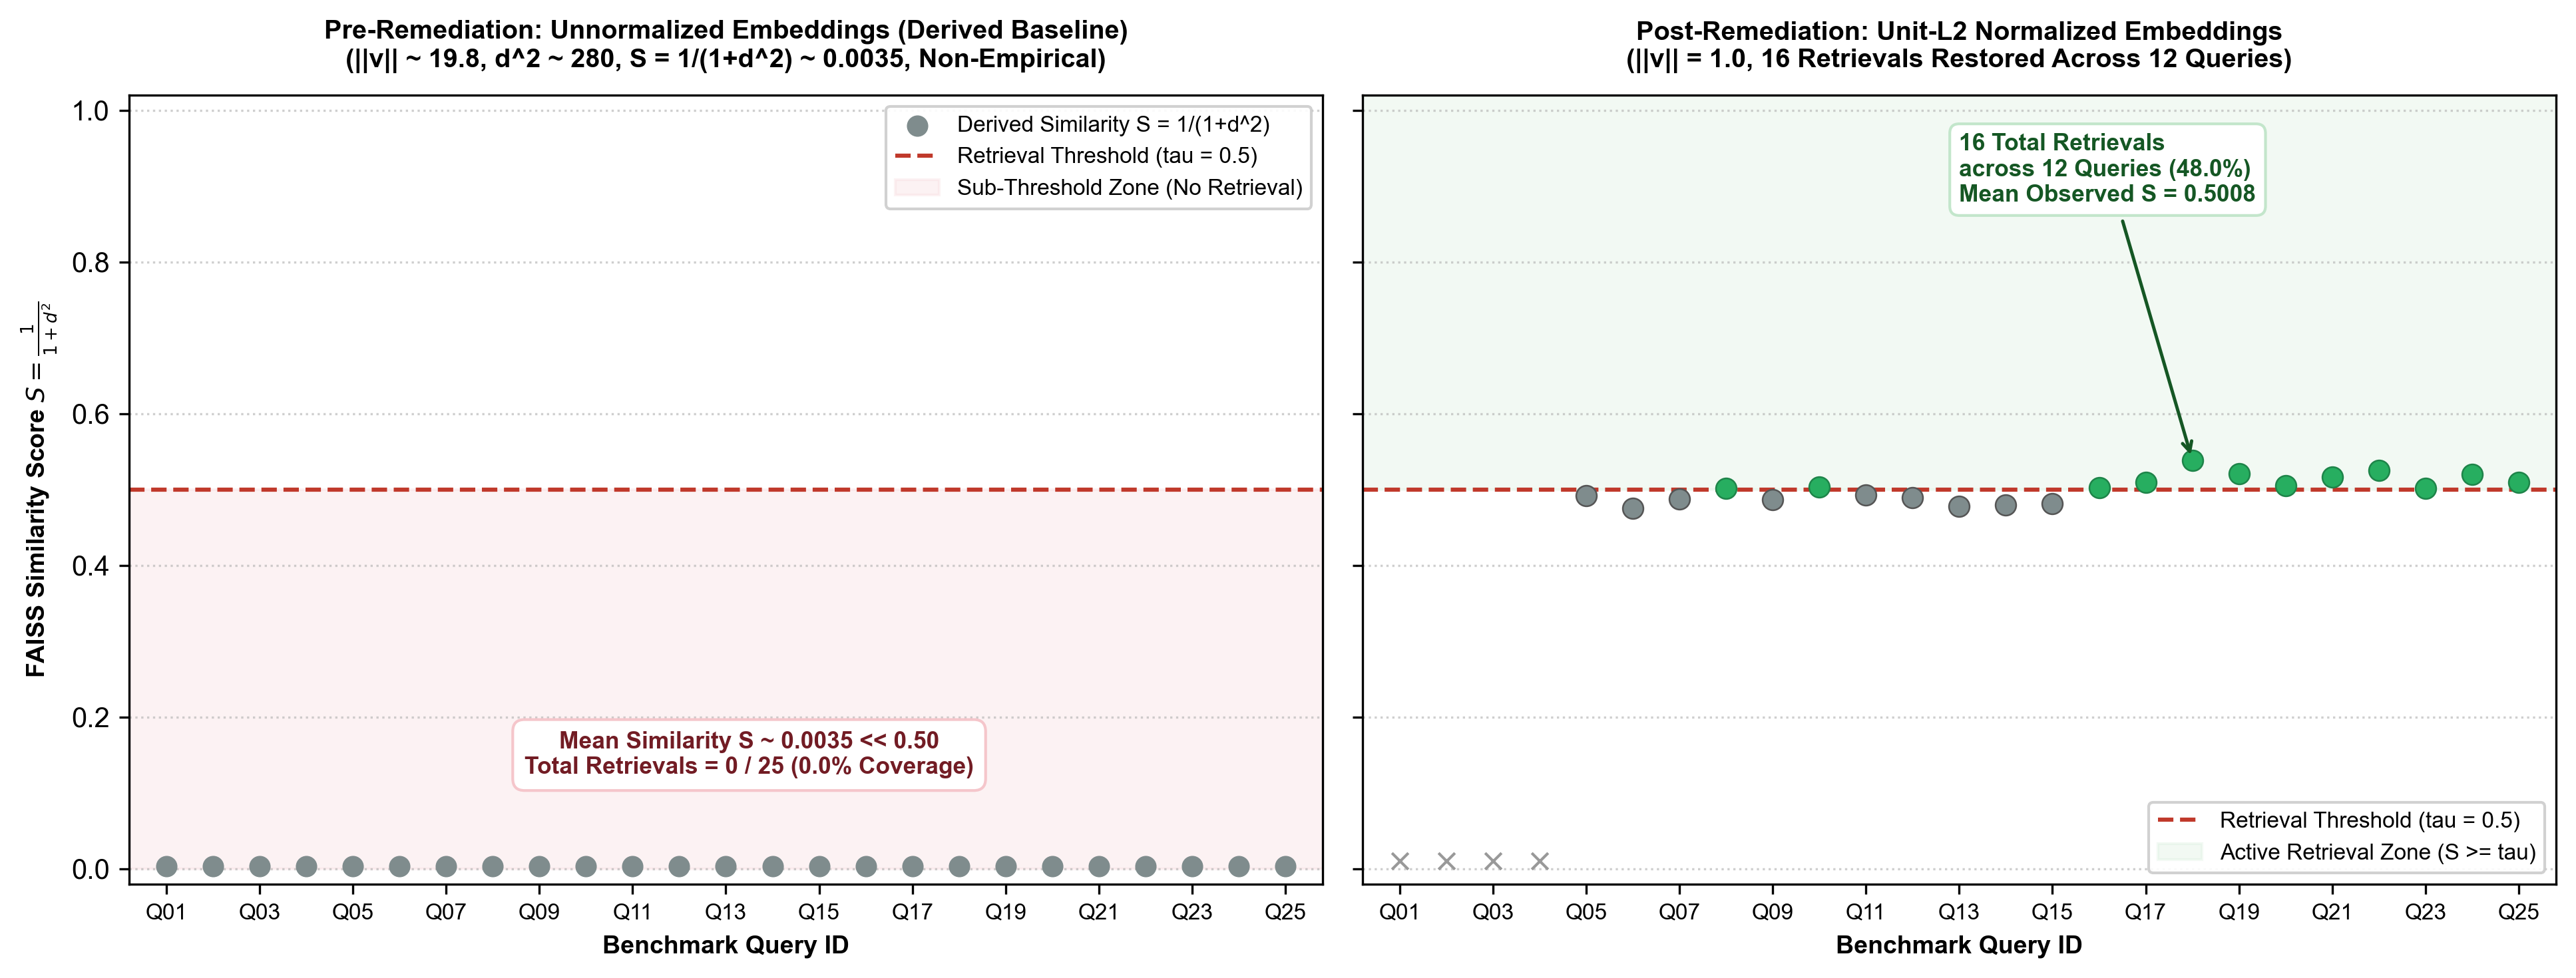
\includegraphics[width=\textwidth]{fig3_retrieval_geometry.png}
\caption{Post-Remediation FAISS Retrieval Telemetry Alongside an Analytical Pre-Remediation Baseline. Left: Analytical geometric calculation for unnormalized vectors ($S = 1/(1+d^2) \approx 0.0035 < \tau = 0.50$; not an executed benchmark run). Right: Observed Mode 4 telemetry under unit-$L_2$ normalization showing 16 retrieval events across 12 distinct queries per run (48.0\% coverage; store empty on Q01--Q04).}
\label{fig:retrieval_geometry}
\end{figure*}

\begin{table*}[t]
\centering
\caption{Benchmark Results Across Six Experimental Configurations (Descriptive Mean $\pm$ Sample SD Over Three Runs; 450 Query-Level Evaluations)}
\label{tab:results}
\footnotesize
\setlength{\tabcolsep}{0pt}
\renewcommand{\arraystretch}{1.03}
\begin{tabular*}{\textwidth}{@{\extracolsep{\fill}}l c c c c c c@{}}
\toprule
\textbf{Experimental Mode} & \textbf{ExecAcc (\%)} & \textbf{ExecSucc (\%)} & \textbf{Retries ($K$)} & \textbf{Latency (ms)} & \textbf{Tokens} & \textbf{Store Size}\textsuperscript{*} \\
\midrule
Mode 1 (Zero-Shot) & $60.00 \pm 0.00$ & $80.00 \pm 0.00$ & $0.00 \pm 0.00$ & $4,859.70 \pm 7.98$ & $360.57 \pm 0.37$ & $0$ \\
Mode 2 (Stateless Self-Correction) & $68.00 \pm 0.00$ & $96.00 \pm 0.00$ & $0.28 \pm 0.00$ & $6,441.56 \pm 105.51$ & $503.72 \pm 0.42$ & $0$ \\
Mode 3 (Naive Vector RAG) & $68.00 \pm 0.00$ & $92.00 \pm 0.00$ & $0.00 \pm 0.00$ & $6,776.25 \pm 34.40$ & $558.28 \pm 0.00$ & $23$ \\
Mode 4 (Full ARMG) & $68.00 \pm 0.00$ & $96.00 \pm 0.00$ & $0.37 \pm 0.05$ & $9,000.59 \pm 184.33$ & $602.85 \pm 28.49$ & $3$ \\
Mode 5 (ARMG $-$ Neg Constraints) & $68.00 \pm 0.00$ & $96.00 \pm 0.00$ & $0.32 \pm 0.00$ & $8,768.48 \pm 100.30$ & $530.97 \pm 0.40$ & $4$ \\
Mode 6 (ARMG with $\lambda = 0.0$) & $68.00 \pm 0.00$ & $96.00 \pm 0.00$ & $0.28 \pm 0.00$ & $8,507.98 \pm 73.15$ & $542.27 \pm 0.39$ & $3$ \\
\bottomrule
\end{tabular*}
\vspace{2.0pt}
\begin{minipage}{\textwidth}
\footnotesize \textsuperscript{*}Each mode reflects 3 runs $\times$ 25 queries $= 75$ query-level evaluations. Store size is the terminal per-run vector count, which was invariant across all three runs within each mode.
\end{minipage}
\end{table*}

\subsection{Finding A: Within-Episode Repair Lifts Executability More Than Relational Execution Accuracy}
Comparing Mode 2 with Mode 1 (Table~\ref{tab:results}) measures stateless execution-guided repair. Mode 1 achieved 80.00\% PostgreSQL execution success (60/75; failing Q04, Q11, Q13, Q15, and Q17 in every run) and 60.00\% relational execution accuracy (45/75). Appending raw PostgreSQL driver exceptions in Mode 2 repaired four of those five failures (Q04, Q13, Q15, and Q17, each in 1 retry, while Q11 exhausted 3 retries, totaling 7 retries per run or $0.2800$ retries/query), raising $\text{ExecSucc}$ to 96.00\% (72/75). However, $\text{ExecAcc}$ rose only to 68.00\% (51/75): Q04 and Q13 matched the gold relation after repair, whereas Q15 and Q17 executed cleanly while returning relationally incorrect window outputs (Fig.~\ref{fig:exec_gap}).

\begin{figure}[t]
\centering
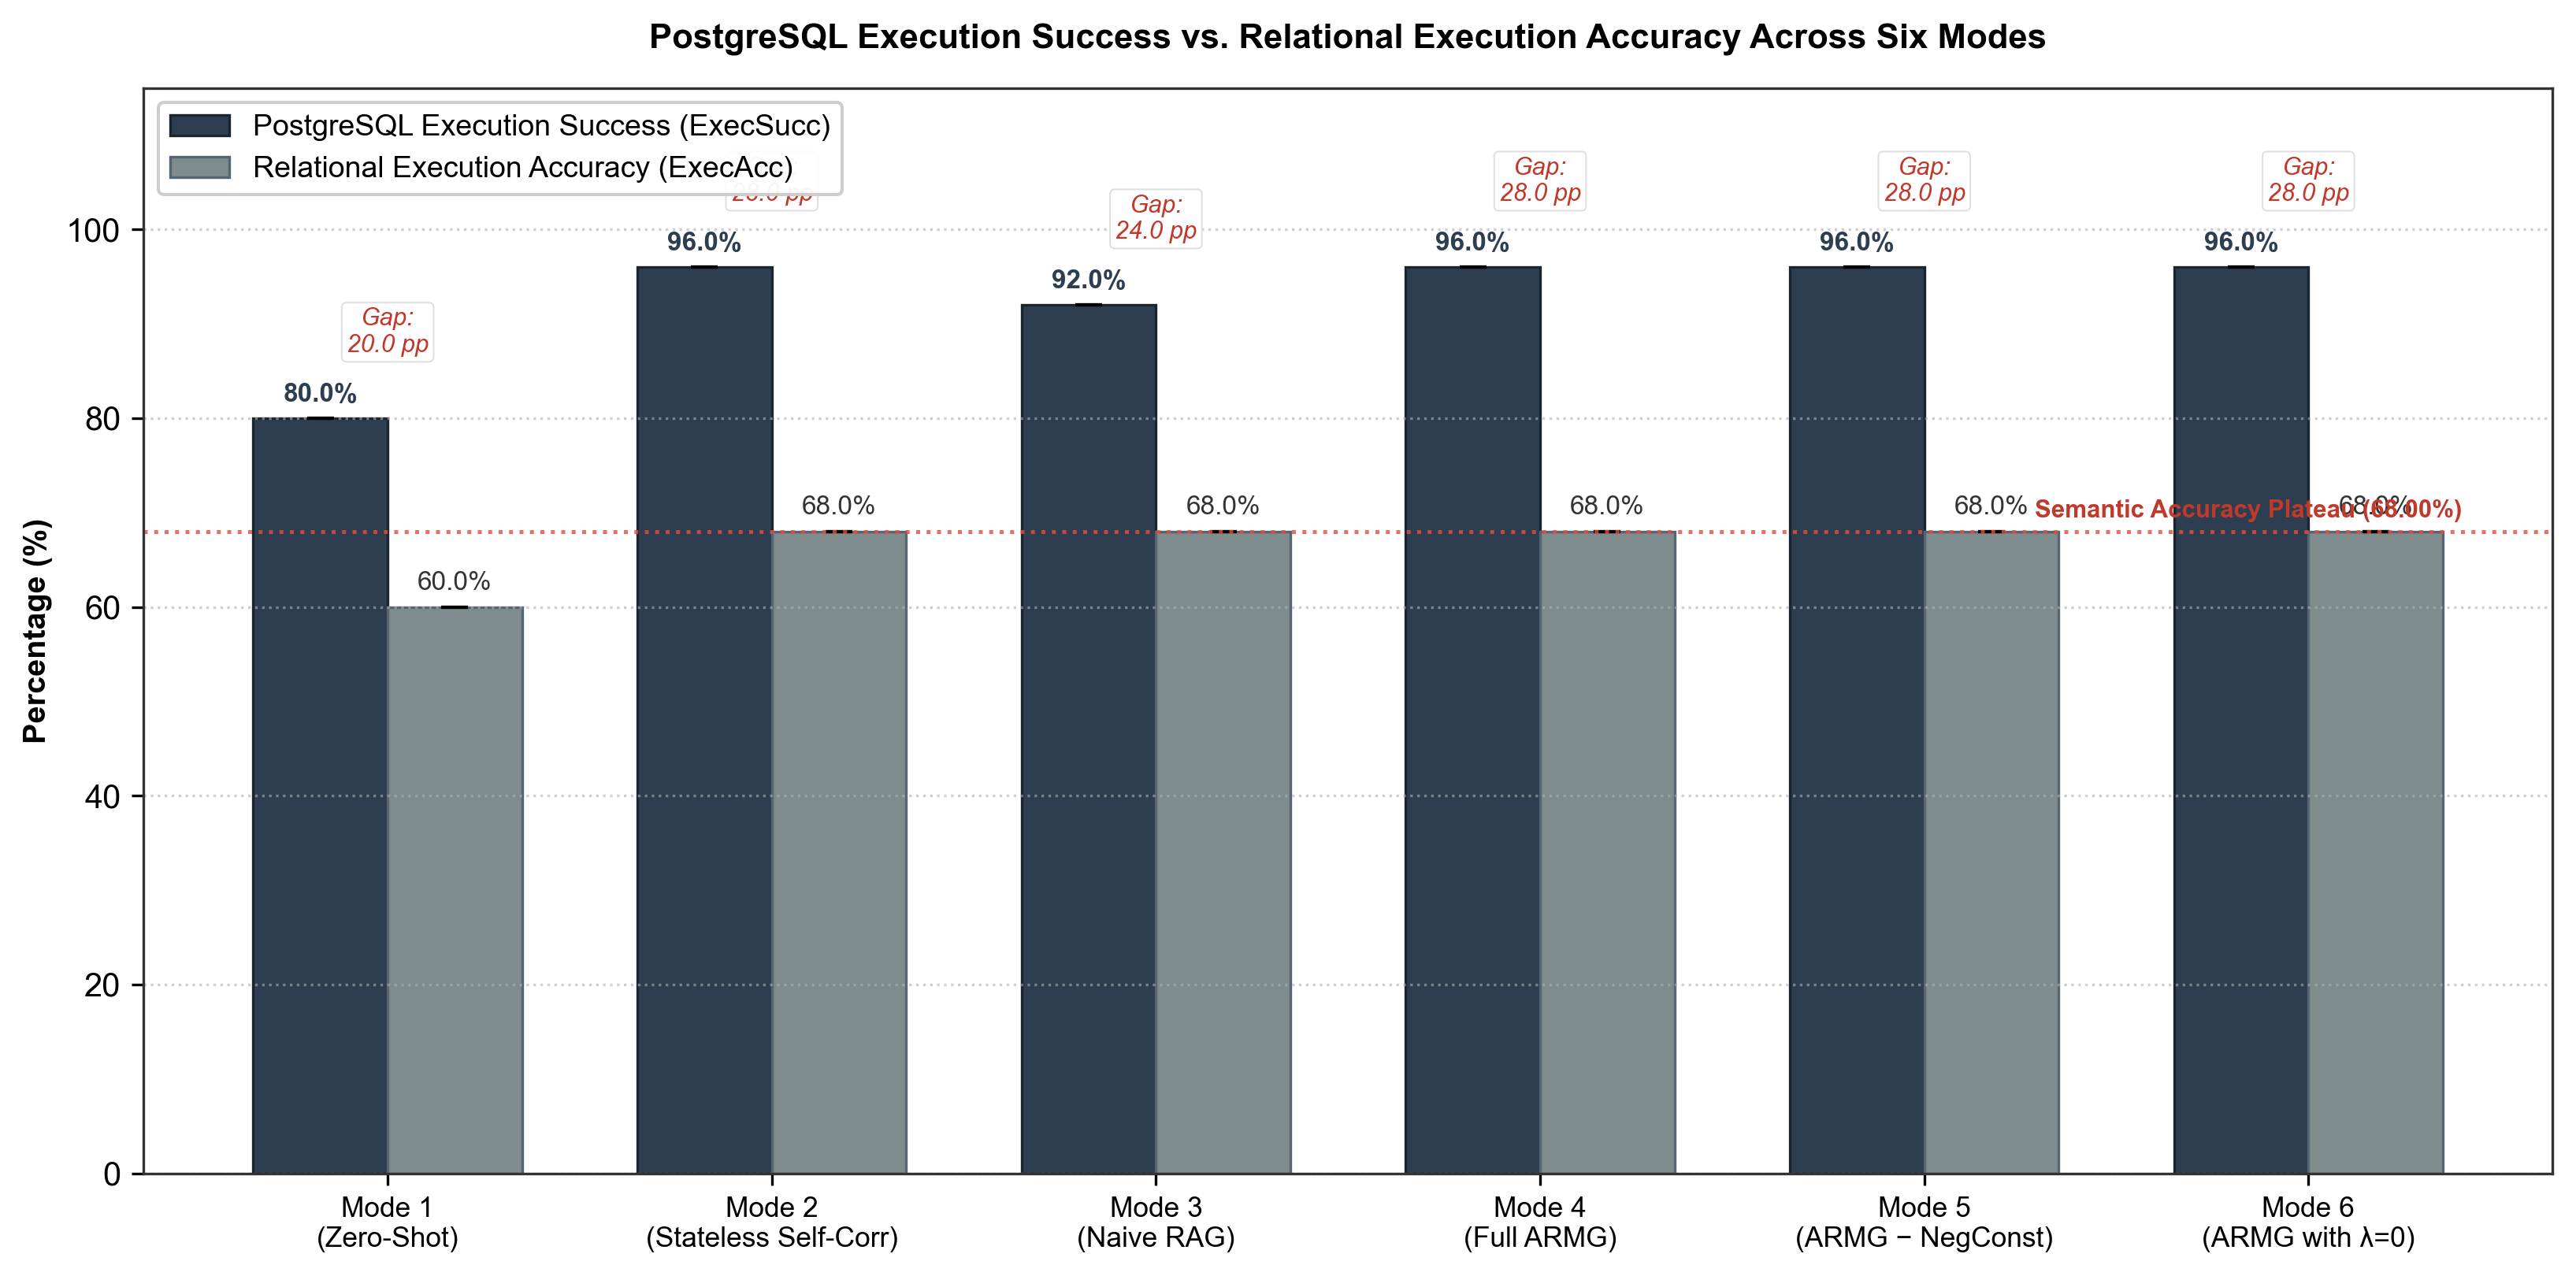
\includegraphics[width=\columnwidth]{fig4_execsucc_execacc.png}
\caption{PostgreSQL Execution Success ($\text{ExecSucc}$) vs. Relational Execution Accuracy ($\text{ExecAcc}$) across six experimental modes ($n = 3$ runs per mode). Relational execution accuracy plateaus at 68.00\% across Modes 2--6 despite 96.00\% execution success in all repair-enabled modes.}
\label{fig:exec_gap}
\end{figure}

\subsection{Finding B: Full ARMG Matched Stateless Repair in Accuracy While Increasing Operational Cost}
Table~\ref{tab:tradeoff} and Fig.~\ref{fig:tradeoff} present the central comparison between Full ARMG (Mode 4) and stateless self-correction (Mode 2). Both configurations achieved 96.00\% PostgreSQL execution success (72/75) and 68.00\% relational execution accuracy (51/75), failing execution only on Q11 and failing relational equivalence on the same seven executable queries in all three runs. Relative to Mode 2, Mode 4 required 33.33\% more retries ($0.3733$ vs. $0.2800$ per query), 19.68\% more tokens ($602.85$ vs. $503.72$ per query), and 39.73\% higher end-to-end latency ($9,000.59$~ms vs. $6,441.56$~ms per query). Because only whole-query wall-clock latency was recorded, $+2,559.03$~ms is reported strictly as an observed end-to-end overhead without attributing shares to embedding calls, FAISS search, graph transitions, or extra repair generations. ARMG was therefore neither more accurate nor more efficient than stateless repair on this benchmark.

\begin{table*}[t]
\centering
\caption{Operational Trade-Off Profile: Mode 4 (Full ARMG) vs. Mode 2 (Stateless Self-Correction)}
\label{tab:tradeoff}
\footnotesize
\setlength{\tabcolsep}{5pt}
\renewcommand{\arraystretch}{1.03}
\begin{tabularx}{\textwidth}{@{}>{\raggedright\arraybackslash}p{3.6cm} r r c c >{\raggedright\arraybackslash}X@{}}
\toprule
\textbf{Evaluation Dimension} & \textbf{Mode 2} & \textbf{Mode 4} & \textbf{Absolute Delta} & \textbf{Relative Delta} & \textbf{Measured Observation and Scope} \\
\midrule
Mean Repair Retries ($K$) & 0.2800 & 0.3733 & $+0.0933$ retries & $+33.33\%$ & Driven by extra retries on Q08 (all 3 runs) and Q19 (seeds 123, 999) \\
Mean Token Expenditure & 503.72 & 602.85 & $+99.13$ tokens & $+19.68\%$ & Reflects longer prompts and extra repair generations; split unmeasured \\
PostgreSQL Execution Success & $96.00\%$ & $96.00\%$ & $0.00\text{ pp}$ & $0.00\%$ & Identical 72/75 execution successes (only Q11 failed in all runs) \\
End-to-End Latency & $6,441.56\text{ ms}$ & $9,000.59\text{ ms}$ & $+2,559.03\text{ ms}$ & $+39.73\%$ & Observed whole-query wall-clock delta; sub-node latencies untimed \\
Relational Execution Accuracy & $68.00\%$ & $68.00\%$ & $0.00\text{ pp}$ & $0.00\%$ & Identical 51/75 accurate evaluations across the same 17 queries per run \\
\bottomrule
\end{tabularx}
\vspace{2.0pt}
\begin{minipage}{\textwidth}
\footnotesize \textsuperscript{*}Percentage-point differences (pp) and relative percentage changes (\%) are distinguished explicitly.
\end{minipage}
\end{table*}

\begin{figure}[t]
\centering
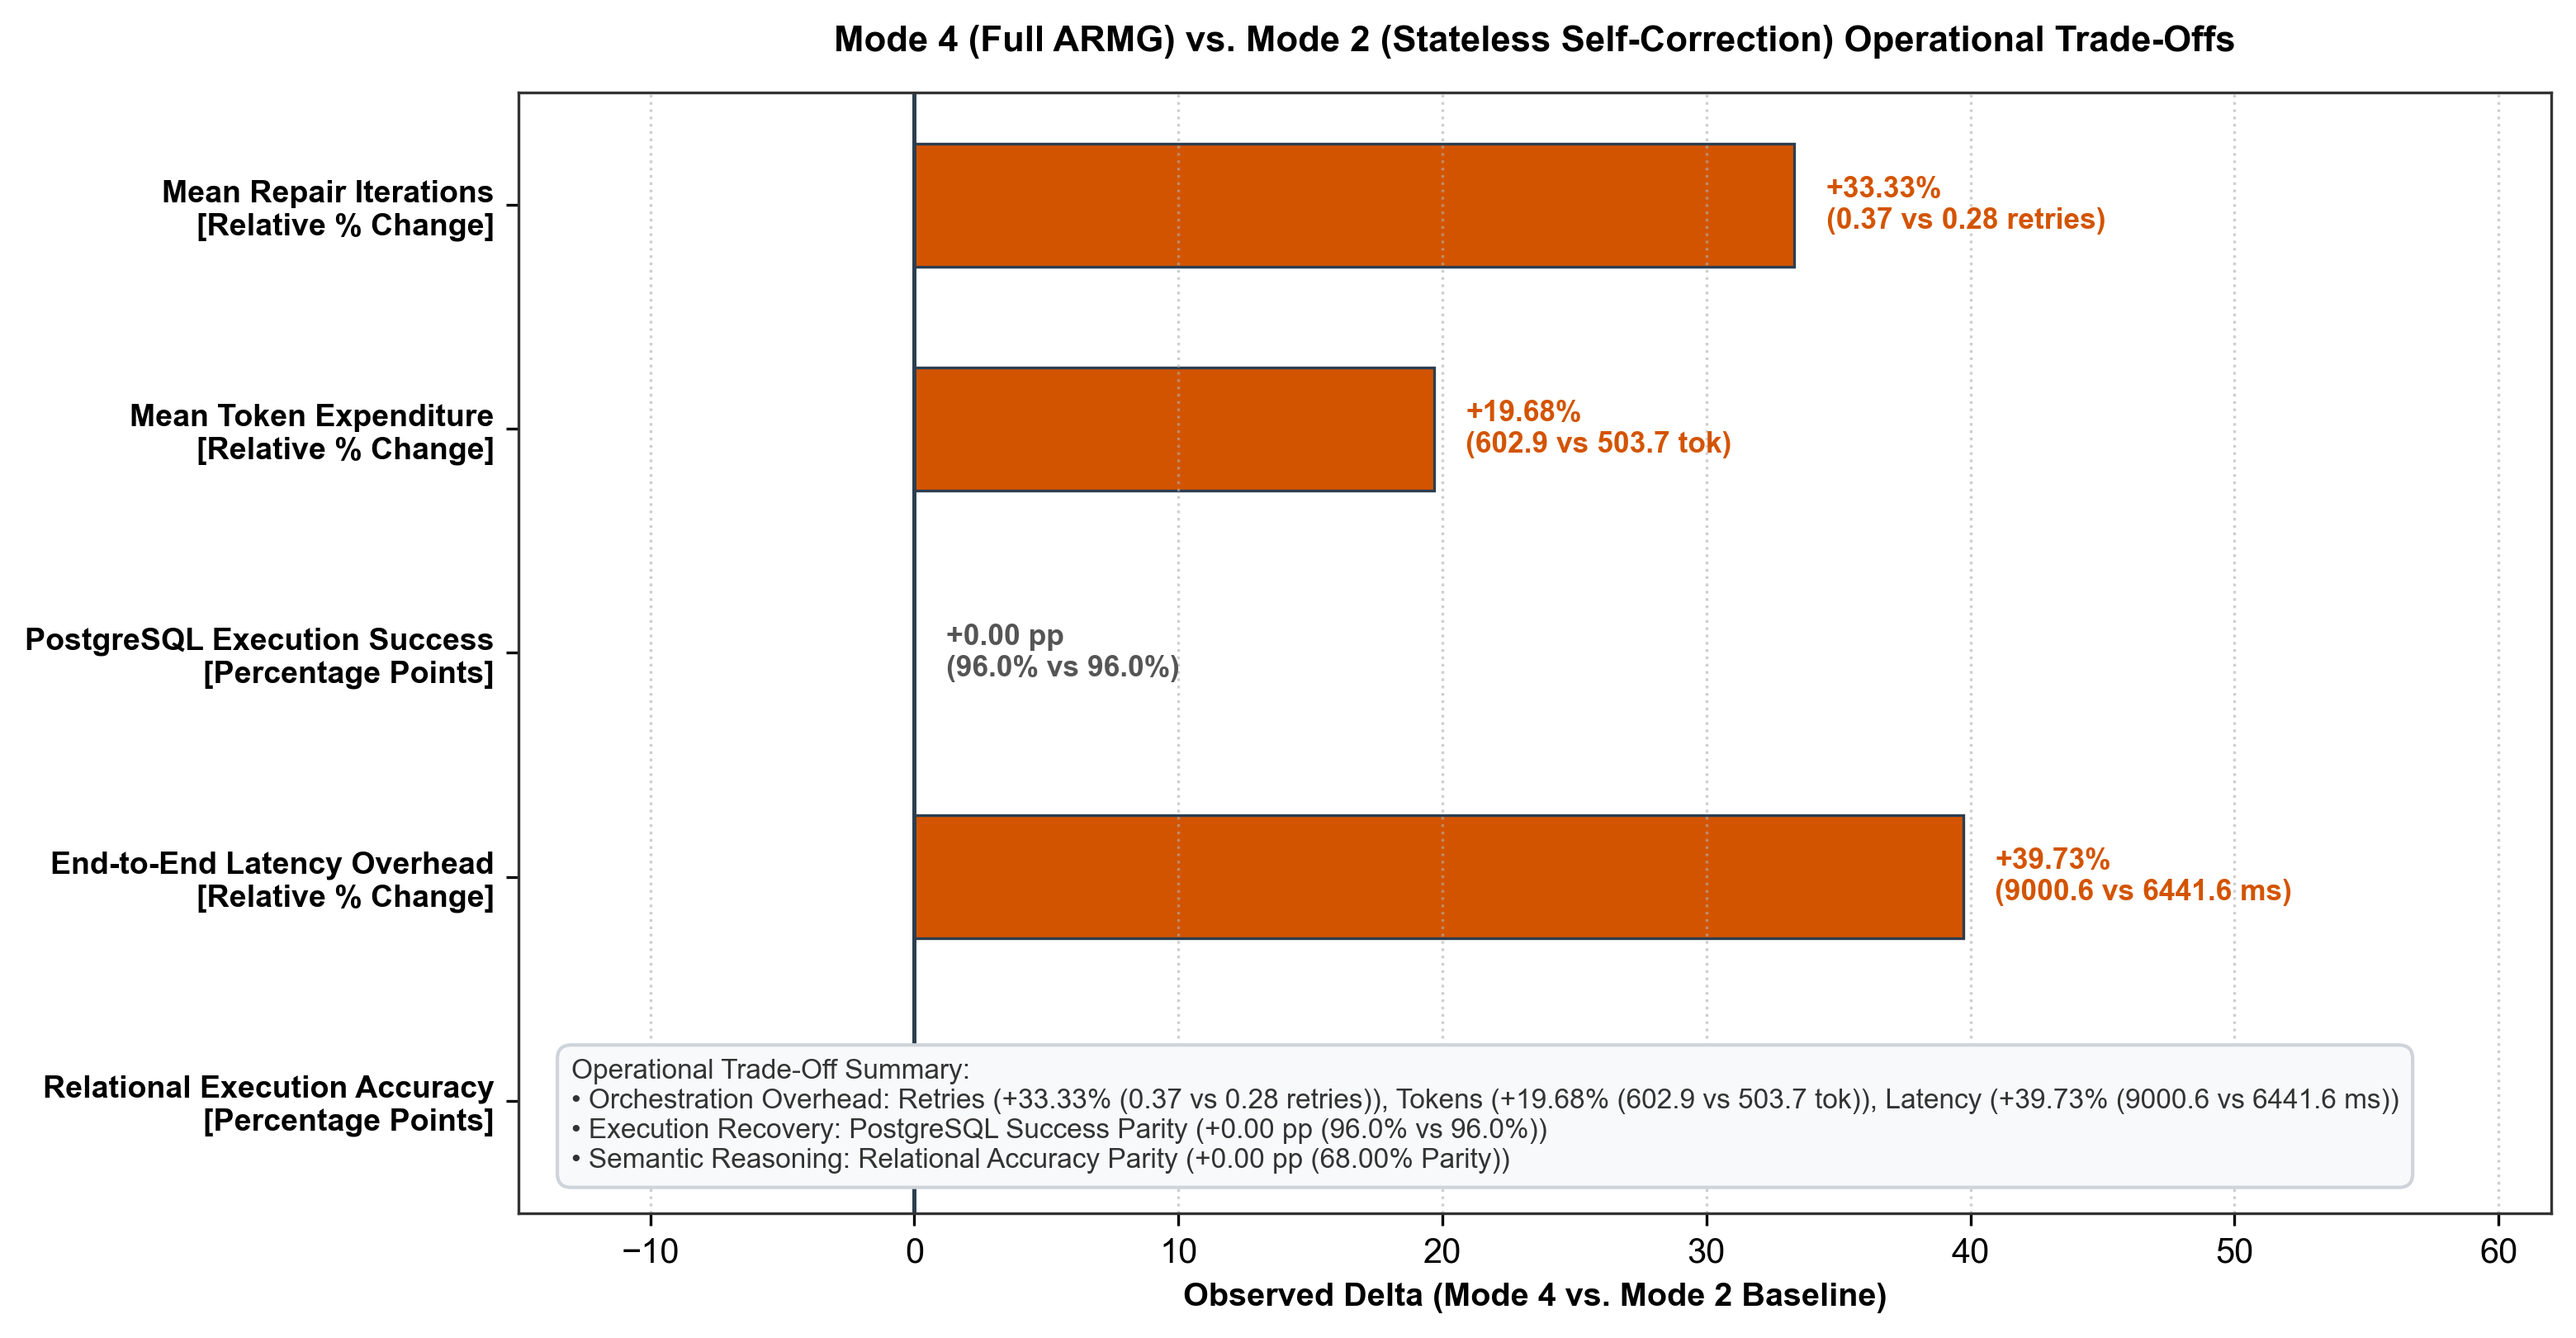
\includegraphics[width=\columnwidth]{fig5_tradeoff.png}
\caption{Mode 2 vs. Mode 4 Operational Trade-Off Profile. Relative to stateless self-correction, Full ARMG incurred $+33.33\%$ mean retries, $+19.68\%$ tokens, and $+39.73\%$ end-to-end latency, with PostgreSQL execution success (96.00\%) and relational execution accuracy (68.00\%) unchanged.}
\label{fig:tradeoff}
\end{figure}

\subsection{Finding C: Mutual Exclusion Bounded Store Growth Without Isolating Governance on Accuracy}
Across the 25-query sequence, Mode 3 stored every executable question--SQL pair (23/25 per run, failing Q04 and Q15 on its single $K=0$ attempt) to accumulate 23 entries (92.00\% $\text{ExecSucc}$, 68.00\% $\text{ExecAcc}$). Mode 4 admitted repair rules only when initial execution failed, repair succeeded ($K \ge 1$), and $M_{\text{applied}} = \emptyset$---occurring at Q04 (\texttt{mem-f5e66b70}, store size 1), Q13 (\texttt{mem-4ff9e3d8}, store size 2, $S = 0.4780 < \tau$), and Q15 (store size 3, $S = 0.4811 < \tau$)---and held store size invariant at three entries from Q15 through Q25 across all runs (Fig.~\ref{fig:memory_growth}; Table~\ref{tab:fig6_validation}). Subsequent repairs with applied memories reinforced existing rules while suppressing new admission (Q08 reinforcing \texttt{mem-f5e66b70} and Q17 reinforcing \texttt{mem-4ff9e3d8} in all runs, plus Q19 in seeds 123 and 999), while first-attempt successes ($K=0$) left the store unchanged. Because Mode 3 also omits iterative repair, Mode 3 versus Mode 4 supports the observed store-growth difference (23 vs. 3 entries) rather than isolating governance's effect on accuracy.

\begin{figure}[t]
\centering
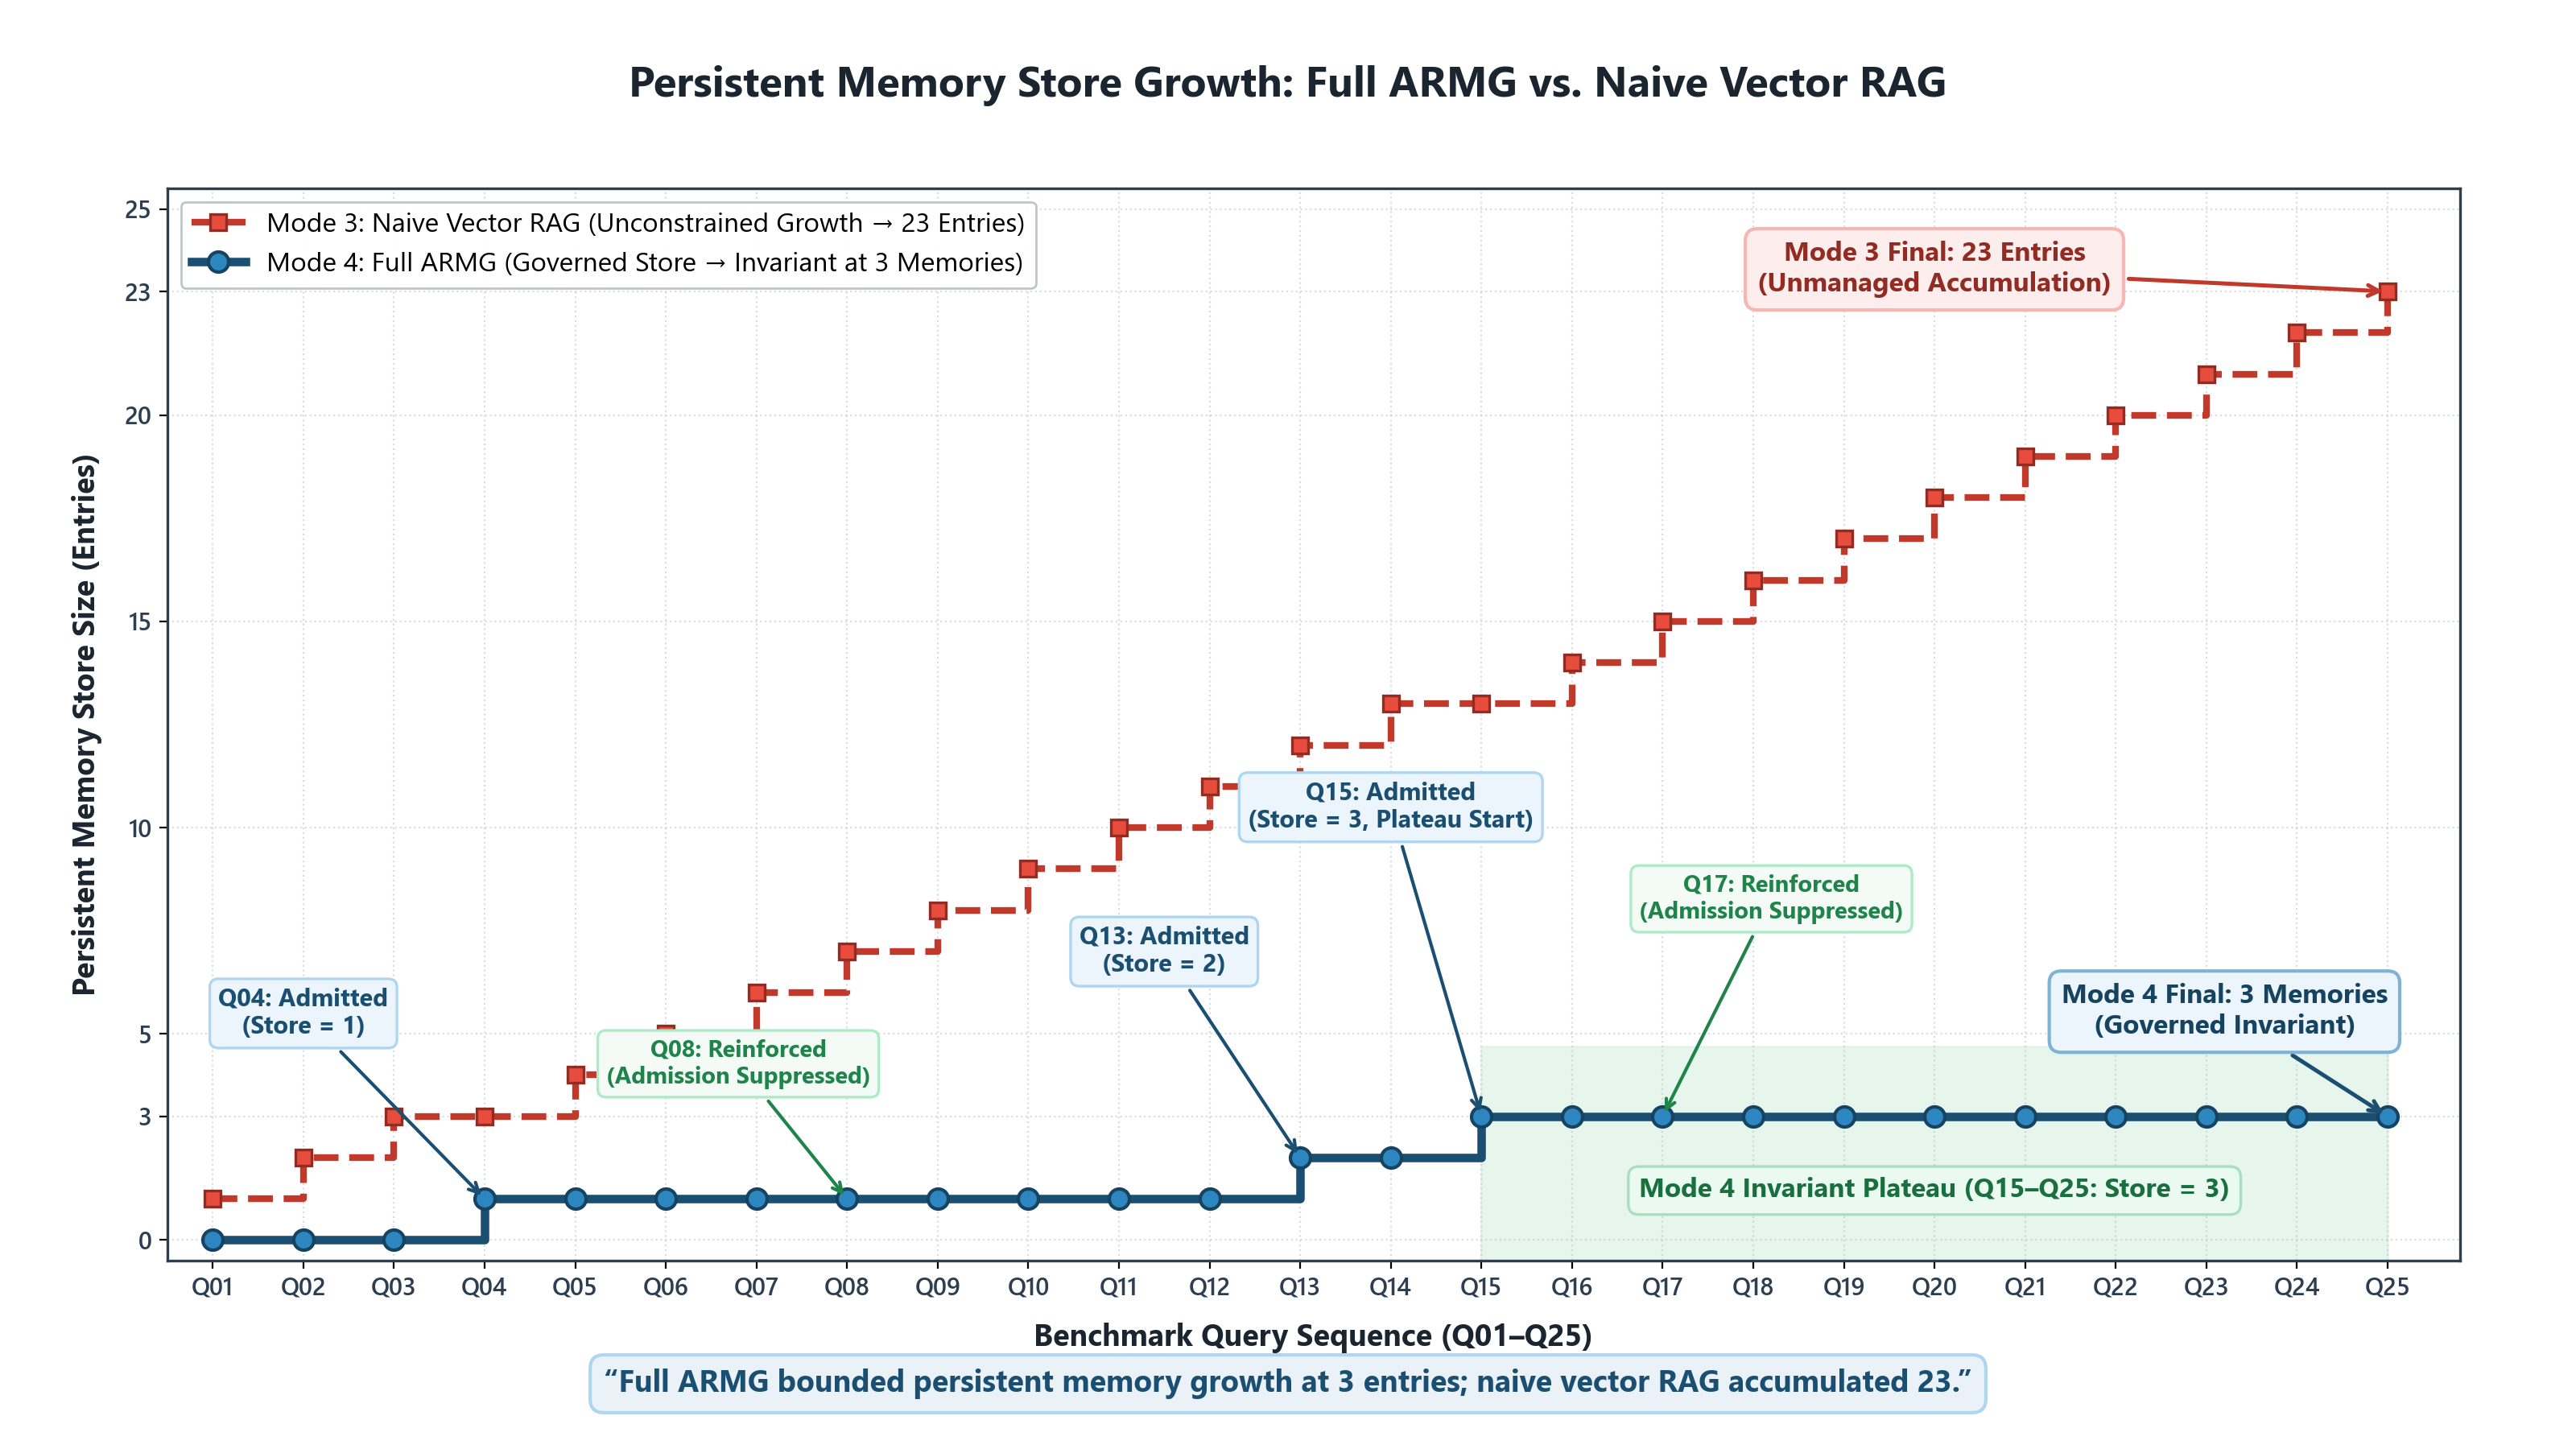
\includegraphics[width=\columnwidth]{fig6_memory_growth.png}
\caption{Persistent Memory Store Growth: Full ARMG (Mode 4) vs. Naive Vector RAG (Mode 3). Mutual exclusion between applied-memory updates and new admission held the Mode 4 store at exactly 3 memories from Q15 through Q25, whereas append-only Mode 3 accumulated 23 entries.}
\label{fig:memory_growth}
\end{figure}

\subsection{Finding D: Query-Level Behavior on Q08, Q11, and Q19}
\textbf{Q08 (retrieval followed by one retry).} Mode 2 solved Q08 on Attempt~1 ($K=0$) in all runs. Mode 4 retrieved \texttt{mem-f5e66b70} ($S = 0.5017$), failed Attempt~1, succeeded on Attempt~2 after one repair retry ($K=1$) with the same relationally accurate result across all three runs, and reinforced \texttt{mem-f5e66b70}. Modes 5 and 6 solved Q08 on Attempt~1 ($K=0$).

\textbf{Q11 (join-plan failure in Modes 1, 2, 4, 5, and 6 vs. few-shot execution in Mode 3).} On Q11, Mode 1 ($K=0$) failed its single attempt, and the repair-enabled modes (Modes 2, 4, 5, and 6) exhausted their three-retry budget (four attempts), repeatedly attempting to join \texttt{dim\_time} directly to \texttt{dim\_geography} instead of bridging through \texttt{fact\_sales\_performance}. Mode 4 rejected the failed episode under \texttt{TERMINAL\_FAILURE\_NOT\_ADMITTED}. Mode 3 ($K=0$) executed Q11 using retrieved few-shot SQL examples from Q06--Q10 (Table~\ref{tab:fig6_validation}), confirming that Q11 reflects a limitation of our single-hop Tier~4 diagnostic hints on a multi-table join plan rather than an inherent impossibility for retrieval-assisted SQL generation.

\textbf{Q19 (extra retries without resolving missing column or rounding).} Mode 2 executed Q19 on Attempt~1 ($K=0$) in all runs. Mode 4 retrieved one memory ($S = 0.5211$), executed on Attempt~1 ($K=0$) in seed 42, and used two repair retries ($K=2$) to reach an executable query in seeds 123 and 999 (reinforcing the applied memory), yet every final query still omitted the base-revenue column and two-decimal rounding. In the absence of counterfactual memory-masking ablations, these extra retries on Q08 and Q19 represent empirical correlations rather than definitive causal artifacts of memory injection.

\subsection{Ablation Interpretations}
\label{sec:ablation}
\textbf{Negative-constraint prompt block (Mode 4 vs. Mode 5).} Removing \texttt{[STRICT REPAIR CONSTRAINTS]} changed retry counts and store size (4 vs. 3) without changing $\text{ExecSucc}$ (96.00\%) or $\text{ExecAcc}$ (68.00\%); thus, negative constraints did not improve relational execution accuracy in this benchmark. Across 75 evaluations, Mode 4 logged 28 retries: 21 base retries across Q04 (3), Q11 (9), Q13 (3), Q15 (3), and Q17 (3), plus 3 retries on Q08 and 4 retries on Q19 ($28/75 = 0.3733$). Mode 5 logged 0 retries on Q08 and Q19 (7 fewer retries), but on Q22 emitted non-existent \texttt{sales\_amount} on Attempt~1 and succeeded on Attempt~2 after one retry ($K=1$) in each run (3 added retries, totaling $24/75 = 0.3200$), admitting a fourth memory at Q22 because $M_{\text{applied}} = \emptyset$.

\textbf{Decay parameter (Mode 4 vs. Mode 6).} Mode 6 ($\lambda = 0.0$) matched Mode 4 on $\text{ExecSucc}$ (96.00\%), $\text{ExecAcc}$ (68.00\%), and store size (3) while recording $0.2800$ retries/query ($21/75$) and $542.27$ tokens/query. As established in Section~\ref{sec:decay_authoritative}, because the live benchmark duration was far too short to exercise multi-day decay, these observed cost and retry differences cannot be attributed to the decay mechanism.

\section{Semantic Failure Analysis}
\label{sec:semantic}
Mode 4 executed 72 of 75 query-level evaluations successfully (96.00\%), but only 51 matched the gold result set (68.00\%). The 21-evaluation gap (28.00 percentage points) corresponds to seven distinct benchmark queries---Q05, Q14, Q15, Q17, Q18, Q19, and Q25---that were executable on PostgreSQL but relationally incorrect across all three runs (and across Modes 2, 4, 5, and 6; Table~\ref{tab:divergent_queries}).

Rather than grouping these cases under a generic label, Table~\ref{tab:divergent_queries} documents the exact SQL construct mismatch and why PostgreSQL accepted each query without raising an exception. On Q05, Q14, Q18, and Q25 (plus Q19 in Mode 2 and seed-42 Mode 4), the initial candidate was legal PostgreSQL syntax ($K=0$), so Nodes~7--10 never ran. On Q15, Q17, and seeds-123/999 Q19, the repair loop activated on an initial execution error ($K \ge 1$) and exited as soon as the regenerated query executed cleanly, leaving the non-cumulative aggregation on Q15, altered row structure on Q17, and missing base-revenue column and rounding on Q19 unflagged. While larger models may construct complex window frames differently \cite{wei2022emergent}, our single-model results show directly why exception-gated repair misses executable queries that compute the wrong relation.

\begin{table*}[t]
\centering
\caption{SQL-Level Breakdown of the Seven Executable-but-Inaccurate Queries in Mode 4 (21 Query-Level Evaluations Across Three Runs)}
\label{tab:divergent_queries}
\footnotesize
\setlength{\tabcolsep}{3.5pt}
\renewcommand{\arraystretch}{1.04}
\begin{tabularx}{\textwidth}{@{}c >{\raggedright\arraybackslash}p{3.3cm} >{\raggedright\arraybackslash}p{3.5cm} >{\raggedright\arraybackslash}p{2.8cm} >{\raggedright\arraybackslash}p{2.3cm} >{\raggedright\arraybackslash}X@{}}
\toprule
\textbf{Query} & \textbf{Gold Query Specification} & \textbf{Reported SQL Failure} & \textbf{Why Execution Still Succeeded} & \textbf{First Comparator Check Failed} & \textbf{Repair Loop Activated?} \\
\midrule
Q05 & Quarterly net profit in 2025 ordered by \texttt{calendar\_quarter} & Required \texttt{ORDER BY} clause omitted & Ordering is optional in SQL \texttt{SELECT} syntax & C4 (ordered row sequence) & No ($K=0$) \\
Q14 & Product revenue with projected \texttt{RANK() OVER (ORDER BY gross\_revenue DESC)} column & Required \texttt{RANK()} output missing; used plain \texttt{ORDER BY} & A sorted query without a rank column is valid SQL & C2 (column count mismatch) & No ($K=0$) \\
Q15 & Monthly cumulative running total via ordered window frame & Cumulative running total replaced by ordinary monthly \texttt{GROUP BY} & \texttt{GROUP BY} executes without computing a cumulative window & C5 (tuple aggregate values) & Yes ($K=1$, fixed initial error) \\
Q17 & Monthly lag series via \texttt{LAG()} over ordered months & Extra grouping attribute changed the \texttt{LAG()} result structure & Legal SQL syntax while returning the wrong row structure & C2 (row count mismatch) & Yes ($K=1$, with applied memory) \\
Q18 & Category-partitioned rank via \texttt{RANK() OVER (PARTITION BY category ...)} & Global ranking used instead of category-partitioned ranking & Unpartitioned global window expression is valid SQL & C5 (rank integer values) & No ($K=0$) \\
Q19 & Category, base revenue sum, and \texttt{ROUND(..., 2)} percentage share & Base revenue column and required two-decimal rounding omitted & Ratio expression is executable without base column or rounding & C2 (column count failed first) & Seeds 123, 999: yes ($K=2$); seed 42: no ($K=0$) \\
Q25 & Output columns ordered as \texttt{(market\_type, gross\_revenue, net\_profit)} & Output columns projected in swapped order (\texttt{net\_profit} before \texttt{gross\_revenue}) & SQL does not require projection order to match the gold query & C5 (positional column alignment) & No ($K=0$) \\
\bottomrule
\end{tabularx}
\vspace{2.0pt}
\begin{minipage}{\textwidth}
\footnotesize Comparator checks C1--C5 are defined in Section~\ref{sec:comparator}. On Q19, omitting the base-revenue column failed check C2 before rounding precision was checked in C5.
\end{minipage}
\end{table*}

\section{Discussion}
Our results indicate that runtime memory governance primarily regulates state accumulation rather than boosting semantic accuracy. By admitting diagnostic rules only on queries Q04, Q13, and Q15 and subsequently routing recurring errors to reinforcement, ARMG froze its vector store at three entries throughout the latter half of the workload. This prevents the memory bloat seen in naive RAG systems. However, mutual exclusion creates an operational blind spot: whenever an existing memory is retrieved and applied during repair, the engine is barred from admitting a newer, more granular diagnostic rule for that failure.

The accuracy results expose a separate limitation of exception-driven repair. Queries Q05, Q14, Q18, and Q25 produced executable SQL on the initial attempt despite missing ordering, ranking, or projection requirements. Because no PostgreSQL exception was raised, the repair loop did not revisit those queries. Queries Q15, Q17, and Q19 entered repair but ultimately produced executable SQL that did not match the gold result set. The current workflow treats a successful PostgreSQL execution as the end of repair; relational comparison is used for evaluation rather than as a further repair trigger.

Because PostgreSQL execution is treated as the terminal success condition, the pipeline lacks the semantic ground truth needed to catch valid-syntax logic errors. Memory governance successfully controls how operational knowledge accumulates, but it cannot compensate for silent semantic mistakes. Breaking through this accuracy ceiling will require integrating post-execution relational assertions or schema graph traversal directly into the feedback loop, while isolating the effect of retrieved memories from the other mechanisms in Full ARMG.

\section{Limitations and Threats to Validity}
\label{sec:limitations}
Each methodological constraint bounds the conclusions that our evidence can support:
\begin{enumerate}
\item \textbf{Single synthetic four-table schema (2,000 rows, 25 queries)}: rules out generalizing store-growth or accuracy findings to wide enterprise warehouses or cross-domain benchmarks such as Spider \cite{yu2018spider} and BIRD \cite{li2023bird}.
\item \textbf{Single 7B local model}: rules out extrapolating failure patterns, admission rates, or window-function errors to larger open-weights or frontier models.
\item \textbf{Greedy decoding, $n = 3$ repeated runs, and unknown Mode 4 Q19 variation}: restricts statistics to descriptive summaries rather than significance tests, and leaves Mode 4's 0-vs-2 retry difference on Q19 unresolved in the retained v1.0 records.
\item \textbf{Fixed query order and absent counterfactual memory masking}: makes retrieval dependent on the Q01--Q25 order, prevents causal attribution of Q08 and Q19 retries to retrieved memories, and prevents Mode 4 vs. Mode 2 (or Mode 3 vs. Mode 4) from isolating persistent memory governance as a single causal variable.
\item \textbf{No component-level latency timers}: prevents attributing Mode 4's $+2,559.03$~ms latency overhead across embedding calls, FAISS search, SQLGlot parsing, graph orchestration, and extra LLM calls.
\item \textbf{Short live benchmark duration and unvalidated dual time weighting}: rules out claiming any live retrieval benefit from multi-day decay or from elapsed time entering utility twice (Section~\ref{sec:decay_authoritative}).
\item \textbf{Manual heuristic weights and non-selective numerical admission threshold}: because $\text{Utility}_0 = \theta_{\text{admit}} = 0.25$ under fixed priors and candidate-scoring weights use hardcoded sales rules without sensitivity tuning, neither parameter set can be claimed as optimal or domain-general.
\item \textbf{Heuristic validators and separated safety test scopes}: rule-based intent matching, heuristic constraint extraction, the 33-case AST audit, and the post-v1.0 unit and integration tests validate only their tested cases outside the frozen 450-evaluation benchmark and do not establish universal security or protection against valid-\texttt{SELECT} resource exhaustion.
\end{enumerate}

\section{Future Work}
Five targeted extensions follow directly from these bounds: (1) run counterfactual memory-masking ablations in Mode 4 on Q08 and Q19 by suppressing \texttt{mem-f5e66b70} and \texttt{mem-4ff9e3d8} at Node~3 while holding the remaining prompt structure fixed; (2) log full serialized prompts, backend states, and token logits to resolve Mode 4's Q19 run-to-run variation; (3) add per-node timers around Node~3, Node~4, and Node~5 to decompose the 2,559.03~ms latency delta; (4) extend Tier~4 diagnosis to compute multi-hop foreign-key paths across central fact tables for Q11-class dimension-join errors; and (5) evaluate larger models and multi-schema workloads over multi-day intervals alongside sensitivity sweeps on $\tau$, $\theta_{\text{admit}}$, and $\lambda$.

\section{Conclusion}
Across 18 sequential runs of 25 queries on one synthetic four-table PostgreSQL warehouse, Full ARMG and stateless self-correction achieved the same execution success (96.00\%) and relational execution accuracy (68.00\%). ARMG held its persistent repair-rule store at three entries from Q15 through Q25, compared with 23 entries in the append-only baseline. Relative to stateless repair, however, ARMG required 33.33\% more retries, 19.68\% more tokens, and 39.73\% higher end-to-end latency. The results support bounded memory growth and the effectiveness of the tested safety controls within their respective evaluation scopes, but they do not establish an accuracy or efficiency gain from governed memory. Broader conclusions require controlled memory-masking experiments, component-level timing, longer-duration decay evaluation, and tests across additional schemas and models.

\appendix
\section{Numerical Validation Tables Underlying Primary Diagrams}

Tables~\ref{tab:fig3_validation}--\ref{tab:fig6_validation} report the exact numerical values plotted in Figs.~\ref{fig:retrieval_geometry}--\ref{fig:memory_growth}. Workspace paths in Table~\ref{tab:figure_validation_matrix} document the internal project CSV logs and plotting scripts from which these summaries were compiled; plotted values can be audited directly from the tables below, while re-executing raw per-seed aggregations requires the project code-and-data archive.

\begin{table*}[t]
\centering
\caption{Numerical Data Underlying the FAISS Retrieval Geometry Analysis (Fig.~\ref{fig:retrieval_geometry})}
\label{tab:fig3_validation}
\footnotesize
\setlength{\tabcolsep}{0pt}
\renewcommand{\arraystretch}{1.03}
\begin{tabular*}{\textwidth}{@{\extracolsep{\fill}}l c c c@{}}
\toprule
\textbf{Query} & \textbf{Post-Remediation Similarity $S$} & \textbf{Threshold Condition ($\tau = 0.50$)} & \textbf{Post-Remediation Retrieval Events} \\
\midrule
Q01 & -- & Store Empty & No (0) \\
Q02 & -- & Store Empty & No (0) \\
Q03 & -- & Store Empty & No (0) \\
Q04 & -- & Store Empty & No (0) \\
Q05 & 0.4917 & $S < \tau$ & No (0) \\
Q06 & 0.4755 & $S < \tau$ & No (0) \\
Q07 & 0.4875 & $S < \tau$ & No (0) \\
Q08 & 0.5017 & $S \ge \tau$ & Yes (1) \\
Q09 & 0.4866 & $S < \tau$ & No (0) \\
Q10 & 0.5031 & $S \ge \tau$ & Yes (1) \\
Q11 & 0.4932 & $S < \tau$ & No (0) \\
Q12 & 0.4895 & $S < \tau$ & No (0) \\
Q13 & 0.4780 & $S < \tau$ & No (0) \\
Q14 & 0.4801 & $S < \tau$ & No (0) \\
Q15 & 0.4811 & $S < \tau$ & No (0) \\
Q16 & 0.5023 & $S \ge \tau$ & Yes (1) \\
Q17 & 0.5091 & $S \ge \tau$ & Yes (3) \\
Q18 & 0.5388 & $S \ge \tau$ & Yes (3) \\
Q19 & 0.5211 & $S \ge \tau$ & Yes (1) \\
Q20 & 0.5050 & $S \ge \tau$ & Yes (1) \\
Q21 & 0.5163 & $S \ge \tau$ & Yes (1) \\
Q22 & 0.5258 & $S \ge \tau$ & Yes (1) \\
Q23 & 0.5016 & $S \ge \tau$ & Yes (1) \\
Q24 & 0.5196 & $S \ge \tau$ & Yes (1) \\
Q25 & 0.5100 & $S \ge \tau$ & Yes (1) \\
\bottomrule
\end{tabular*}
\vspace{3.0pt}
\begin{minipage}{\textwidth}
\scriptsize \textbf{Analytical Baseline vs. Observed Telemetry Summary} (source path: \url{benchmark/retrieval_telemetry.csv}; threshold $\tau = 0.50$): (1) \emph{Illustrative Analytical Baseline}: unnormalized \texttt{nomic-embed-text} vectors ($\Vert\mathbf{v}\Vert_2 \approx 19.8, d^2 \approx 280$) yield $S = 1/(1+d^2) \approx 0.0035 \ll \tau = 0.50$ (0/25 retrievals), serving as an analytical geometric reference rather than an executed run. (2) \emph{Observed Post-Remediation Telemetry}: unit-$L_2$ normalized vectors produced 16 retrieval events across 12 distinct queries per run (48.0\% coverage); Q01--Q04 record no score because the store was initially empty.
\end{minipage}
\end{table*}

\begin{table*}[t]
\centering
\caption{Numerical Data Underlying PostgreSQL Execution Success vs. Relational Execution Accuracy (Fig.~\ref{fig:exec_gap})}
\label{tab:fig4_validation}
\footnotesize
\setlength{\tabcolsep}{0pt}
\renewcommand{\arraystretch}{1.03}
\begin{tabular*}{\textwidth}{@{\extracolsep{\fill}}l c c c c c c@{}}
\toprule
\textbf{Experimental Mode} & \textbf{ExecSucc (\%)} & \textbf{ExecAcc (\%)} & \textbf{Gap (pp)} & \textbf{PG Successes / 75} & \textbf{Rel. Accurate / 75} & \textbf{Query Evals} \\
\midrule
Mode 1 (Zero-Shot Baseline) & $80.00 \pm 0.00$ & $60.00 \pm 0.00$ & $20.00$ & 60 / 75 & 45 / 75 & 75 \\
Mode 2 (Stateless Self-Correction) & $96.00 \pm 0.00$ & $68.00 \pm 0.00$ & $28.00$ & 72 / 75 & 51 / 75 & 75 \\
Mode 3 (Naive Vector RAG) & $92.00 \pm 0.00$ & $68.00 \pm 0.00$ & $24.00$ & 69 / 75 & 51 / 75 & 75 \\
Mode 4 (Full ARMG) & $96.00 \pm 0.00$ & $68.00 \pm 0.00$ & $28.00$ & 72 / 75 & 51 / 75 & 75 \\
Mode 5 (ARMG $-$ Neg Constraints) & $96.00 \pm 0.00$ & $68.00 \pm 0.00$ & $28.00$ & 72 / 75 & 51 / 75 & 75 \\
Mode 6 (ARMG with $\lambda = 0.0$) & $96.00 \pm 0.00$ & $68.00 \pm 0.00$ & $28.00$ & 72 / 75 & 51 / 75 & 75 \\
\midrule
\textbf{Total Across 18 Runs} & $92.67$ & $66.67$ & $26.00$ & 417 / 450 & 300 / 450 & 450 \\
\bottomrule
\end{tabular*}
\vspace{2.0pt}
\begin{minipage}{\textwidth}
\footnotesize Descriptive mean $\pm$ sample SD across three runs (seeds 42, 123, and 999); each mode contributes 75 query-level evaluations. In Modes 2, 4, 5, and 6, the 21-evaluation difference ($72 - 51$) reflects 7 executable-but-inaccurate queries across 3 runs ($28.00\text{ pp}$).
\end{minipage}
\end{table*}

\begin{table*}[t]
\centering
\caption{Numerical Data Underlying the Operational Trade-Off Profile (Fig.~\ref{fig:tradeoff})}
\label{tab:fig5_validation}
\footnotesize
\setlength{\tabcolsep}{0pt}
\renewcommand{\arraystretch}{1.03}
\begin{tabular*}{\textwidth}{@{\extracolsep{\fill}}l c c c c c@{}}
\toprule
\textbf{Evaluation Metric} & \textbf{Mode 2} & \textbf{Mode 4} & \textbf{Observed Delta} & \textbf{Delta Type} & \textbf{Unit} \\
\midrule
Mean Repair Retries & $0.2800$ & $0.3733$ & $+33.33\%$ & Relative & retries/query \\
Mean Token Expenditure & $503.72$ & $602.85$ & $+19.68\%$ & Relative & tokens/query \\
PostgreSQL Execution Success & $96.00\%$ & $96.00\%$ & $+0.00\text{ pp}$ & Percentage points & pp \\
End-to-End Latency & $6,441.56$ & $9,000.59$ & $+39.73\%$ & Relative & ms \\
Relational Execution Accuracy & $68.00\%$ & $68.00\%$ & $0.00\text{ pp}$ & Percentage points & pp \\
\bottomrule
\end{tabular*}
\vspace{2.0pt}
\begin{minipage}{\textwidth}
\scriptsize Rate-based operational metrics (retries, tokens, latency) are reported as relative percentage changes; $\text{ExecSucc}$ and $\text{ExecAcc}$ are reported as percentage-point differences.
\end{minipage}
\end{table*}

\begin{table*}[t]
\centering
\caption{Numerical Data Underlying Persistent Memory Store Growth (Fig.~\ref{fig:memory_growth}): Seed-42 Run Trace}
\label{tab:fig6_validation}
\footnotesize
\setlength{\tabcolsep}{0pt}
\renewcommand{\arraystretch}{1.03}
\begin{tabular*}{\textwidth}{@{\extracolsep{\fill}} c c c l l @{}}
\toprule
\textbf{Query} & \textbf{Mode 3 Store Size} & \textbf{Mode 4 Store Size} & \textbf{Mode 3 Event} & \textbf{Mode 4 Governance Event (Seed 42)} \\
\midrule
Q01 & 1 & 0 & \texttt{NAIVE\_STORED} & None (Att.~1 Succ, $K=0$) \\
Q02 & 2 & 0 & \texttt{NAIVE\_STORED} & None (Att.~1 Succ, $K=0$) \\
Q03 & 3 & 0 & \texttt{NAIVE\_STORED} & None (Att.~1 Succ, $K=0$) \\
Q04 & 3 & 1 & None (Att.~1 Fail) & \texttt{ADMITTED} (\texttt{mem-f5e66b70}, $K=1$) \\
Q05 & 4 & 1 & \texttt{NAIVE\_STORED} & None (Att.~1 Succ, $K=0$) \\
Q06 & 5 & 1 & \texttt{NAIVE\_STORED} & None (Att.~1 Succ, $K=0$) \\
Q07 & 6 & 1 & \texttt{NAIVE\_STORED} & None (Att.~1 Succ, $K=0$) \\
Q08 & 7 & 1 & \texttt{NAIVE\_STORED} & \texttt{REINFORCED} (\texttt{mem-f5e66b70}, $K=1$) \\
Q09 & 8 & 1 & \texttt{NAIVE\_STORED} & None (Att.~1 Succ, $K=0$) \\
Q10 & 9 & 1 & \texttt{NAIVE\_STORED} & None (Att.~1 Succ, $K=0$) \\
Q11 & 10 & 1 & \texttt{NAIVE\_STORED} & \texttt{REJECTED} (Terminal Fail, $K=3$) \\
Q12 & 11 & 1 & \texttt{NAIVE\_STORED} & None (Att.~1 Succ, $K=0$) \\
Q13 & 12 & 2 & \texttt{NAIVE\_STORED} & \texttt{ADMITTED} (\texttt{mem-4ff9e3d8}, $K=1$) \\
Q14 & 13 & 2 & \texttt{NAIVE\_STORED} & None (Att.~1 Succ, $K=0$) \\
Q15 & 13 & 3 & None (Att.~1 Fail) & \texttt{ADMITTED} (3rd rule, $K=1$) \\
Q16 & 14 & 3 & \texttt{NAIVE\_STORED} & None (Att.~1 Succ, $K=0$) \\
Q17 & 15 & 3 & \texttt{NAIVE\_STORED} & \texttt{REINFORCED} (\texttt{mem-4ff9e3d8}, $K=1$) \\
Q18 & 16 & 3 & \texttt{NAIVE\_STORED} & None (Att.~1 Succ, $K=0$) \\
Q19 & 17 & 3 & \texttt{NAIVE\_STORED} & None in seed 42 ($K=0$); \texttt{REINFORCED} in seeds 123, 999 ($K=2$) \\
Q20 & 18 & 3 & \texttt{NAIVE\_STORED} & None (Att.~1 Succ, $K=0$) \\
Q21 & 19 & 3 & \texttt{NAIVE\_STORED} & None (Att.~1 Succ, $K=0$) \\
Q22 & 20 & 3 & \texttt{NAIVE\_STORED} & None (Att.~1 Succ, $K=0$) \\
Q23 & 21 & 3 & \texttt{NAIVE\_STORED} & None (Att.~1 Succ, $K=0$) \\
Q24 & 22 & 3 & \texttt{NAIVE\_STORED} & None (Att.~1 Succ, $K=0$) \\
Q25 & 23 & 3 & \texttt{NAIVE\_STORED} & None (Att.~1 Succ, $K=0$) \\
\bottomrule
\end{tabular*}
\vspace{3.0pt}
\begin{minipage}{\textwidth}
\scriptsize \textbf{Trajectory Summary} (workspace paths: \url{benchmark/seed42/benchmark_results.csv}, \url{benchmark/seed123/benchmark_results.csv}, \url{benchmark/seed999/benchmark_results.csv}, and \url{manuscript/figures/source/fig6_memory_growth.py}): Across all three Mode 4 runs, store size followed $0 \to 1 \to 2 \to 3$ via admissions at Q04, Q13, and Q15 and remained at 3 from Q15 through Q25; Q08 and Q17 triggered reinforcement in all runs, while Q19 also triggered reinforcement ($K=2$) in seeds 123 and 999. Mode 3 ($K=0$) executed Q11 via few-shot retrieval, failed Q04 and Q15, and reached 23 entries.
\end{minipage}
\end{table*}

\begin{table*}[t]
\centering
\caption{Mapping Between Manuscript Figures, Appendix Validation Tables, and Project Workspace Artifacts}
\label{tab:figure_validation_matrix}
\footnotesize
\setlength{\tabcolsep}{3.5pt}
\renewcommand{\arraystretch}{1.05}
\begin{tabularx}{\textwidth}{@{}>{\raggedright\arraybackslash}p{4.0cm} p{2.0cm} >{\raggedright\arraybackslash}p{4.2cm} p{2.3cm} >{\raggedright\arraybackslash}X@{}}
\toprule
\textbf{Diagram / Chart Title} & \textbf{Validation Table} & \textbf{Internal Workspace Path} & \textbf{Data Scope} & \textbf{Verification Scope} \\
\midrule
FAISS Retrieval Geometry & Table~\ref{tab:fig3_validation} & \url{benchmark/retrieval_telemetry.csv} & 25 queries (Q01--Q25) & Plotted values tabulated in Table~\ref{tab:fig3_validation} \\
PostgreSQL Execution Success vs. Relational Execution Accuracy & Table~\ref{tab:fig4_validation} & \url{benchmark/seed*/benchmark_results.csv} & 6 modes (18 runs; 450 evals) & Aggregated mode statistics tabulated in Table~\ref{tab:fig4_validation} \\
Operational Trade-Off Profile & Table~\ref{tab:fig5_validation} & \url{benchmark/seed*/benchmark_results.csv} & 5 Mode 2 vs. Mode 4 metrics & Exact deltas verifiable from Tables~\ref{tab:results} and~\ref{tab:fig5_validation} \\
Persistent Memory Store Growth & Table~\ref{tab:fig6_validation} & \url{benchmark/seed*/benchmark_results.csv} & 25 sequential queries & Per-query trace tabulated in Table~\ref{tab:fig6_validation} (\url{manuscript/figures/source/fig6_memory_growth.py}) \\
\bottomrule
\end{tabularx}
\vspace{2.0pt}
\begin{minipage}{\textwidth}
\scriptsize Plotted quantities can be audited directly from Tables~\ref{tab:fig3_validation}--\ref{tab:fig6_validation} in this manuscript; regenerating the CSV summaries from raw logs requires the internal project code-and-data archive.
\end{minipage}
\end{table*}

\bibliographystyle{IEEEtran}
\bibliography{\jobname}
\end{document}
